\documentclass{article}
\usepackage{geometry}                % See geometry.pdf to learn the layout options. There are lots.
%\geometry{letterpaper}                   % ... or a4paper or a5paper or ...
%\geometry{landscape}                % Activate for for rotated page geometry
%\usepackage[parfill]{parIEEEabrvskip}    % Activate to begin paragraphs with an empty line rather than an indent
\usepackage{graphicx}
\usepackage{caption}
\usepackage{subcaption}
\usepackage{amssymb}
\usepackage{amsmath}
\usepackage{epstopdf}
\usepackage{amsthm}
\usepackage{authblk}
\DeclareGraphicsRule{.tif}{png}{.png}{`convert #1 `dirname #1`/`basename #1 .tif`.png}

\newtheorem*{mydef}{Definition}
\title{Determinism, Complexity, and Predictability in Computer Performance}


\author[1]{Joshua Garland \thanks{joshua.garland@colorado.edu}}
\author[1]{Ryan James \thanks{ryan.james@colorado.edu}}
\author[1,2]{Elizabeth Bradley \thanks{lizb@colorado.edu}}
\affil[1]{Department of Computer Science\\
  University of Colorado at Boulder\\
  Colorado, USA
}
\affil[2]{Santa Fe Institute\\
  New Mexico, USA
}


%Version 1
%\author{
%  \IEEEauthorblockN{Joshua Garland}
%  \IEEEauthorblockA{Dept. of Computer Science\\
%    University of Colorado at Boulder\\
%    Colorado, USA\\
%    Email: joshua.garland@colorado.edu}
%  \and
%  \IEEEauthorblockN{Ryan G.~James}
%  \IEEEauthorblockA{Complexity Sciences Center \& Dept. of Physics\\
%    University of California at Davis\\
%    California, USA\\
%    Email: rgjames@ucdavis.edu}
%    \and
%      \IEEEauthorblockN{Elizabeth Bradley}
%         \IEEEauthorblockA{Santa Fe Institute \\
%    New Mexico, USA\\
%    }
%  \IEEEauthorblockA{Dept. of Computer Science\\
%    University of Colorado at Boulder\\
%    Colorado, USA\\
%    Email: lizb@colorado.edu}
%  }



 %\author{
 %  \IEEEauthorblockN{
 %    Joshua Garland\IEEEauthorrefmark{1},
 %    Ryan G.~James\IEEEauthorrefmark{1} and
 %    Elizabeth Bradley\IEEEauthorrefmark{1}\IEEEauthorrefmark{2}}
 %  \IEEEauthorblockA{
 %    \IEEEauthorrefmark{1}Dept. of Computer Science
 %    University of Colorado, Boulder, Colorado 80309-0430 USA\\
 %    Email: joshua.garland@colorado.edu, ryan.james@colorado.edu}
 %  \IEEEauthorblockA{
 %    \IEEEauthorrefmark{2}Santa Fe Institute, 1399 Hyde Park Road, Santa Fe, New Mexico 87501  USA\\
 %    Email: lizb@colorado.edu}
 %  % \IEEEauthorblockA{
 %  %   \IEEEauthorrefmark{3}Complexity Sciences Center \& Physics Dept., University of California, Davis, %California 95616 USA\\
%   %   Email: rgjames@ucdavis.edu}
% }

\begin{document}



\maketitle





\begin{abstract}
  Computers are deterministic dynamical systems \cite{mytkowicz09}.
  Among other things, that implies that one should be able to use
  deterministic forecast rules to predict aspects of their behavior.
  That statement is sometimes---but not always---true. The memory and
  processor loads of some simple programs are easy to predict, for
  example, but those of more-complex programs like {\tt gcc} are not.
%%%%%%%%%%%%%%%%%%%%%%
%% I had to change all the \verb|blah| entries because they caused
%% latex to barf if they were in figure captions.  Odd bug.
%%%%%%%%%%%%%%%%%%%%%%
  The goal of this paper is to determine why that is the case. We
  conjecture that, in practice, complexity can effectively overwhelm
  the predictive power of deterministic forecast models. To explore
  that, we build models of a number of performance traces from
  different programs running on different Intel-based computers. We
  then calculate the \emph{permutation entropy}---a temporal entropy
  metric that uses ordinal analysis---of those traces and correlate
  those values against the prediction success.
\end{abstract}

\section{Introduction}
%\begin{it}
%Paragraph on computer performance, including citations to Todd paper
%and summary of the results that indicate that they're deterministic
%nonlinear dynamical systems.  Given that, we should be able to
%predict.  What benefits would accrue if we could do so: power mgmt,
%end world hunger [[this is my primary goal everyday :)]], etc.
%\end{it}

Computers are among the most complex engineered artifacts in current
use.  Modern microprocessor chips contain multiple processing units
and multi-layer memories, for instance, and they use complicated
hardware/software strategies to move data and threads of computation
across those resources.  These features---along with all the others
that go into the design of these chips---make the patterns of their
processor loads and memory accesses highly complex and hard to
predict.  Accurate forecasts of these quantities, if one could
construct them, could be used to improve computer design.  If one
could predict that a particular computational thread would be bogged
down for the next 0.6 seconds waiting for data from main memory, for
instance, one could save power by putting that thread on hold for that
time period (e.g., by migrating it to a processing unit whose clock
speed is scaled back).  Computer performance traces are, however, very
complex.  Even a simple ``microkernel,'' like a three-line loop that
repeatedly initializes a matrix in column-major order, can produce
{\sl chaotic} performance traces \cite{mytkowicz09}, as shown in
Figure~\ref{fig:cache}, and chaos places fundamental limits on
predictability.
%
\begin{figure}[htbp]
   \centering
   \includegraphics[width=0.5\textwidth]{figs/colCacheShort}
   % where an .eps filename suffix will be assumed under latex,
   % and a .pdf suffix will be assumed for pdflatex
   \caption{A small snippet of the L2 cache miss rate of {\tt
       col\_major}, a three-line C program that repeatedly initializes
     a matrix in column-major order, running on an Intel Core
     Duo\textsuperscript{\textregistered}-based machine.  Even this
     simple program exhibits chaotic performance dynamics.}
   \label{fig:cache}
 \end{figure}

The computer systems community has applied a variety of prediction
strategies to traces like this, most of which employ regression.  An
appealing alternative builds on the recently established fact that
computers can be effectively modeled as deterministic nonlinear
dynamical systems \cite{mytkowicz09}.  This result implies the
existence of a deterministic forecast rule for those dynamics.  In
particular, one can use \emph{delay-coordinate embedding} to
reconstruct the underlying dynamics of computer performance, then use
the resulting model to forecast the future values of computer
performance metrics such as memory or processor loads
\cite{josh-ida2011}.  In the case of simple microkernels like the one
that produced the trace in Figure~\ref{fig:cache}, this deterministic
modeling and forecast strategy works very well.  In more-complicated
programs, however, such as speech recognition software or compilers,
this forecast strategy---as well as the traditional methods---break
down quickly.

This paper is a first step in understanding when, why, and how
deterministic forecast strategies fail when they are applied to
deterministic systems.  We focus here on the specific example of
computer performance.  We conjecture that the complexity of traces
from these systems---which results from the inherent dimension,
nonlinearity, and nonstationarity of the dynamics, as well as from
measurement issues like noise, aggregation, and finite data
length---can make those deterministic signals \emph{effectively}
unpredictable.  We argue that \emph{permutation entropy}
\cite{bandt2002per}, a method for measuring the entropy of a
real-valued-finite-length time series through ordinal analysis, is an
effective way to explore that conjecture.  We study four
examples---two simple microkernels and two complex programs from the
SPEC benchmark suite---running on different Intel-based machines.  For
each program, we calculate the permutation entropy of the processor
load (instructions per cycle) and memory-use efficiency (cache-miss
rates), then compare that to the prediction accuracy attainable for
that trace using a simple deterministic model.

% paragraph to appease the theoretician in me
It is worth taking a moment to consider the theoretical possibility of
this task. We are not attempting to predict the state of the CPU at an
arbitrary point in the future --- this, at least with perfect
accuracy, would be tantamount to solving the halting problem. What we
are attempting is to predict aspects or functions of the running of
the CPU: instructions executed per second, cache misses per 100,000
instructions, and similar statistics. Prediction of these quantities
at some finite time in the future, even with perfect accuracy, does
not violate the Rice-Shapiro theorem.

% The rest of the paper is organized as follows.
% Section~\ref{sec:compModel} describes the experimental setup, as well
% as the nonlinear modeling and forecast strategies.  In
% Section~\ref{sec:meaComplex}, we review permutation entropy, calculate
% its value for a number of different computer performance traces, and
% compare the results to the prediction accuracy.  In
% Section~\ref{sec:conc}, we discuss these results and their
% implications in regard to our conjecture, and consider future areas of
% research.

\section{Modeling Computer Performance}\label{sec:compModel}

% took out for space
% \subsection{Reconstructing hidden dynamics}

Delay-coordinate embedding allows one to reconstruct a system's full
state-space dynamics from a \emph{single} scalar time-series
measurement---provided that some conditions hold regarding that data.
Specifically, if the underlying dynamics and the measurement
function---the mapping from the unknown state vector $\vec{X}$ to the
scalar value $x$ that one is measuring---are both smooth and generic,
Takens~\cite{takens} formally proves that the delay-coordinate map
\[
F(\tau,m)(x) = ([x(t) ~ x(t+\tau) ~ \dots ~x(t+m\tau)])
\]
from a $d$-dimensional smooth compact manifold $M$ to ${Re}^{2d+1}$,
where $t$ is time, is a diffeomorphism on $M$---in other words, that
the reconstructed dynamics and the true (hidden) dynamics have the
same topology.

This is an extremely powerful result: among other things, it means
that one can build a formal model of the full system dynamics without
measuring (or even knowing) every one of its state variables.  This is
the foundation of the modeling approach that is used in this paper.
The first step in the process is to estimate values for the two free
parameters in the delay-coordinate map: the delay $\tau$ and the
dimension $m$.  We follow standard procedures for this, choosing the
first minimum in the average mutual information as an estimate of
$\tau$ \cite{fraser-swinney} and using the false-near(est) neighbor
method of \cite{KBA92}, with a threshold of 10\%, to estimate $m$.  A
plot of the data from Figure~\ref{fig:cache}, embedded following this
procedure, is shown in Figure~\ref{fig:embedding}.
\begin{figure}
  \centering
    \includegraphics[width=0.5\textwidth]{figs/3dcolcache}
    \caption{A 3D projection of a delay-coordinate embedding of the trace
from Figure~\ref{fig:cache} with a delay ($\tau$) of 100,000 instructions.
}
\label{fig:embedding}
\end{figure}
%% can cut for space if need be:
The coordinates of each point on this plot are differently delayed
elements of the \verb|col_major| L2 cache miss rate time series
$y(t)$: that is, $y(t)$ on the first axis, $y(t+\tau)$ on the second,
$y(t+2\tau)$ on the third, and so on.
%% ...down to here.
Structure in these kinds of plots---clearly visible in
Figure~\ref{fig:embedding}---is an indication of
determinism\footnote{A deeper analysis of
  Figure~\ref{fig:embedding}---as alluded to on the previous
  page---supports that diagnosis, confirming the presence of a chaotic
  attractor in these cache-miss dynamics, with largest Lyapunov
  exponent $\lambda_1 = 8000 \pm 200$ instructions, embedded in a
  12-dimensional reconstruction space \cite{mytkowicz09}.}.  That
structure can also be used to build a forecast model.

% took out for space
% \subsection{LMA: Using dynamics in forecasting}

Given a nonlinear model of a deterministic dynamical system in the
form of a delay-coordinate embedding like Figure~\ref{fig:embedding},
one can build deterministic forecast algorithms by capturing and
exploiting the geometry of the embedding.  Many techniques have been
developed by the dynamical systems community for this purpose
(e.g.,~\cite{casdagli-eubank92,weigend-book}).  Perhaps the most straightforward
is the ``Lorenz method of analogues'' (LMA), which is essentially
nearest-neighbor prediction in the embedded state
space~\cite{lorenz-analogues}.  Even this simple algorithm---which
builds predictions by finding the nearest neighbor in the embedded
space of the given point, then taking that neighbor's path as the
forecast---works quite well on the trace in Figure~\ref{fig:cache}, as
shown in Figure~\ref{fig:cachePredTS}.
%
\begin{figure}[htbp]
  \centering
    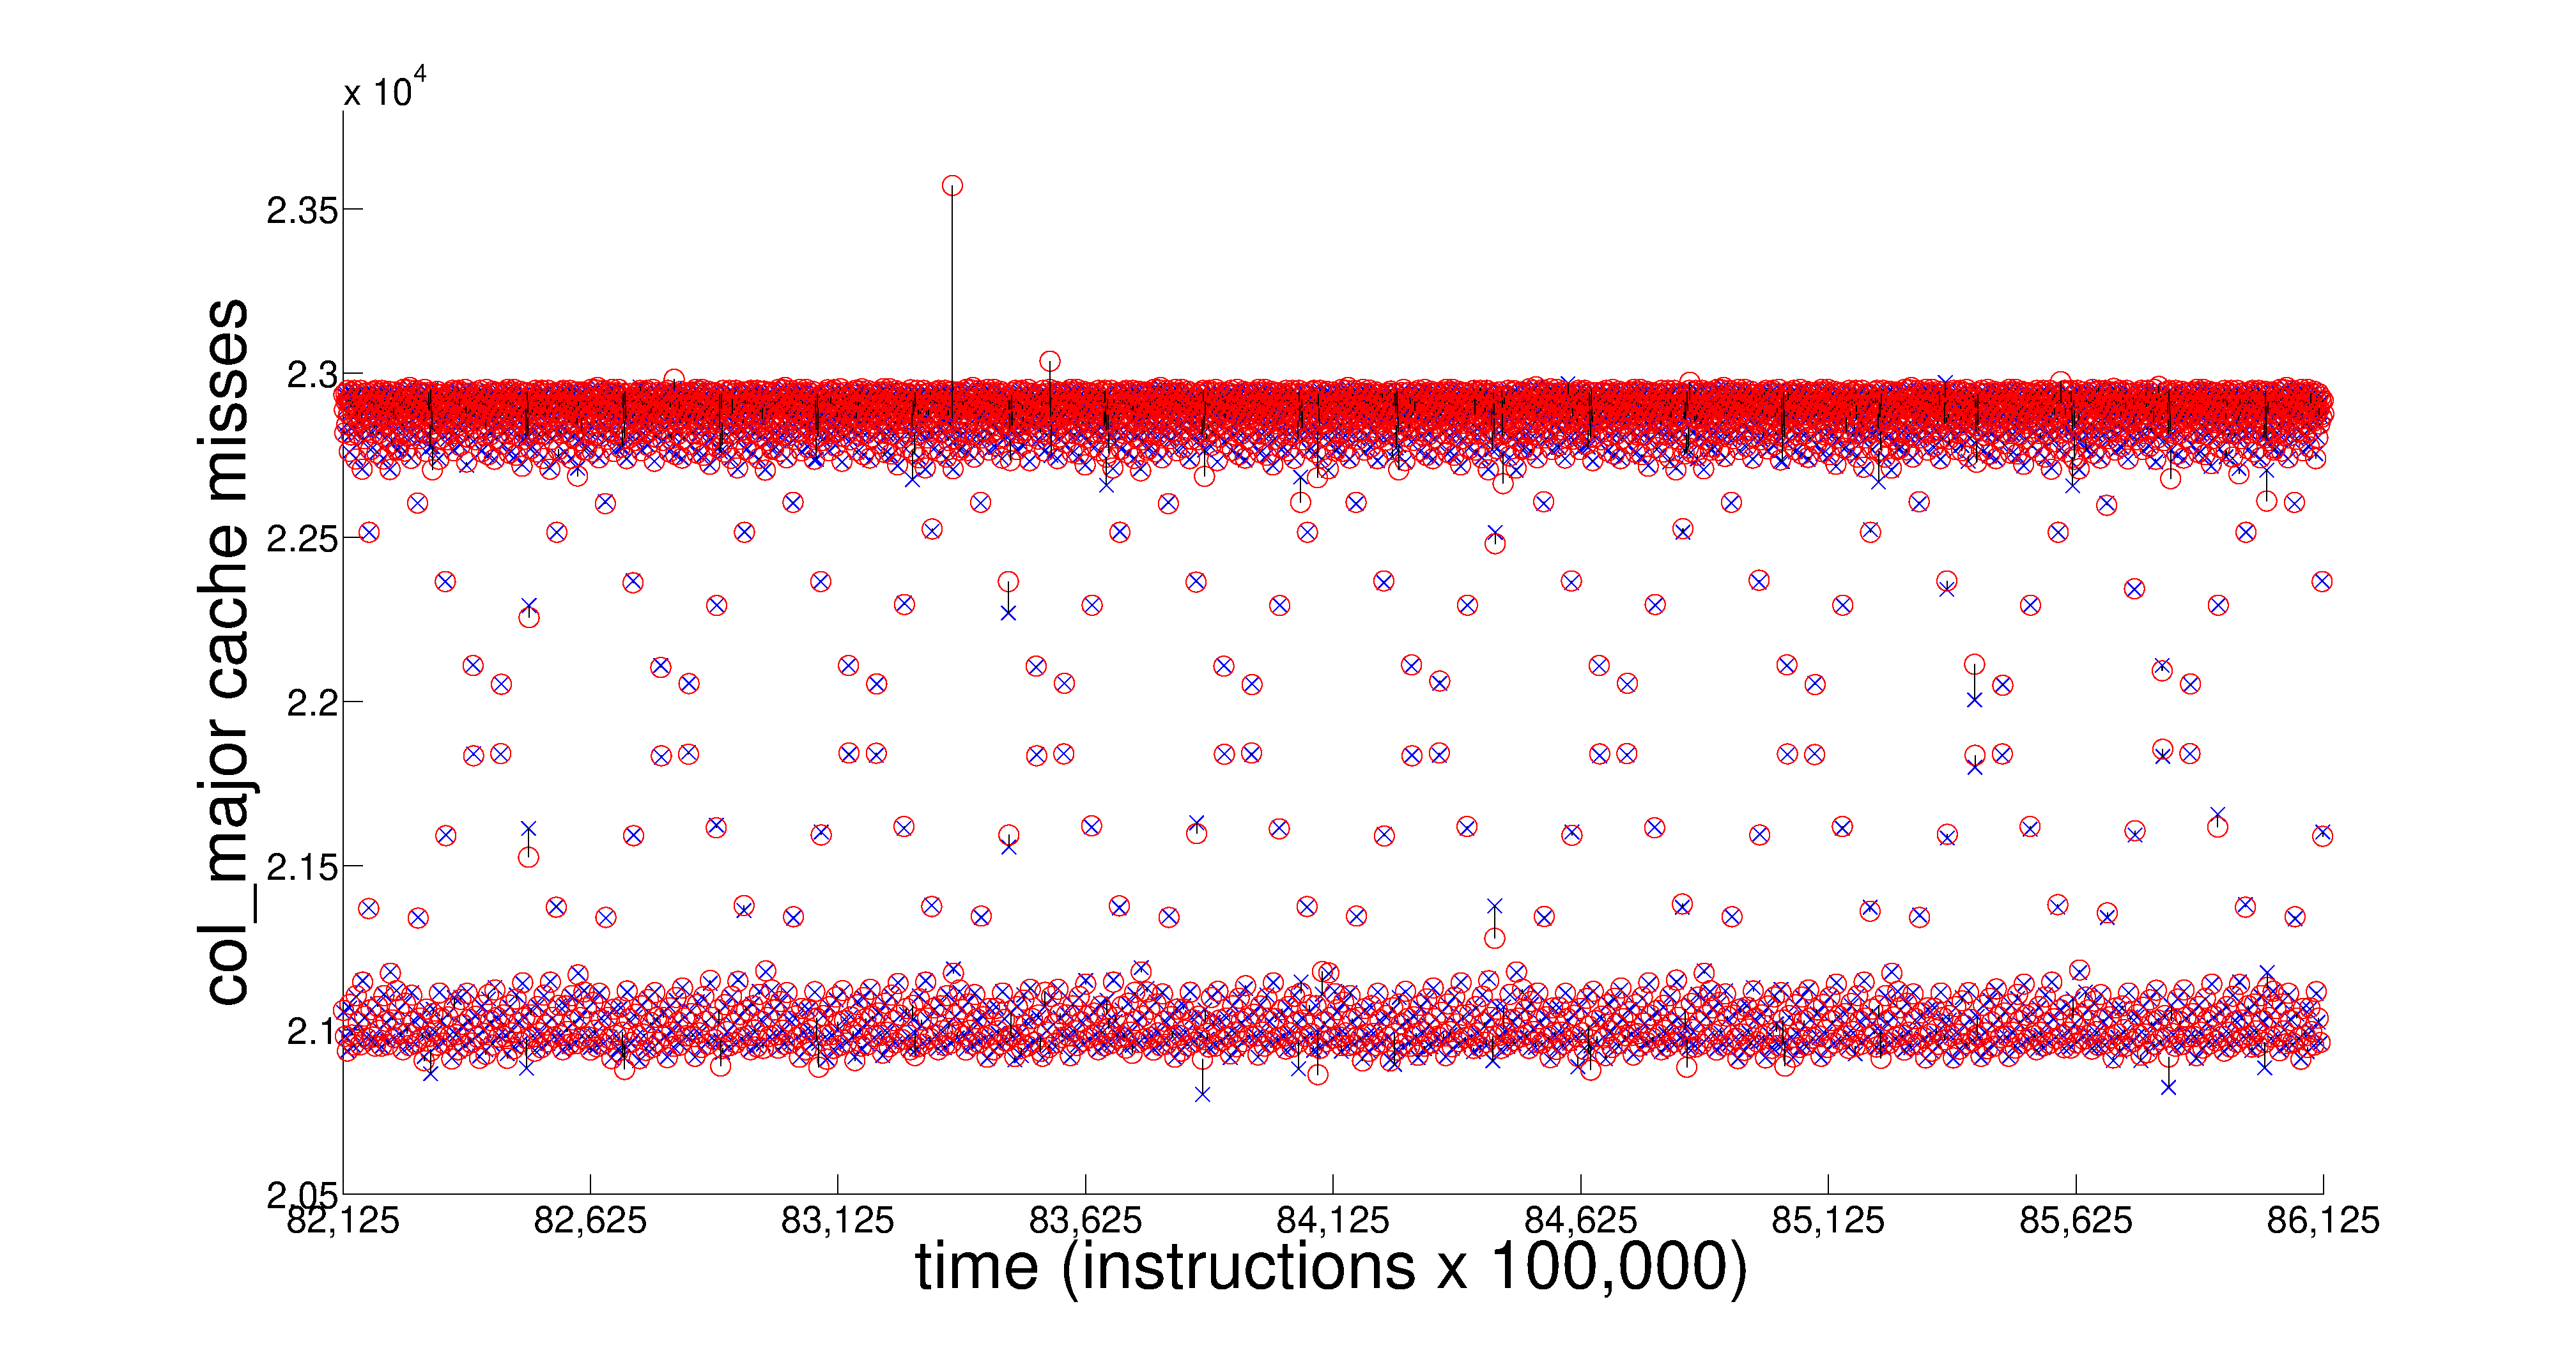
\includegraphics[width=0.5\textwidth]{figs/colCachePredTS}
    \caption{A forecast of the last 4,000 points of the signal in
      Figure~\ref{fig:cache} using an LMA-based strategy on the
      embedding in Figure~\ref{fig:embedding}.  Red circles and blue
      $\times$s are the true and predicted values, respectively;
      vertical bars show where these values differ. }
\label{fig:cachePredTS}
\end{figure}
%
On the other hand, if we use the same approach to forecast the
processor load\footnote{Instructions per cycle, or IPC} of the {\tt
  482.sphinx3} program from the SPEC cpu2006 benchmark suite, running
on an Intel i7\textsuperscript{\textregistered}-based machine, the
prediction is far less accurate; see Figure~\ref{fig:predsphinx}.
%
\begin{figure}[htbp]
  \centering
    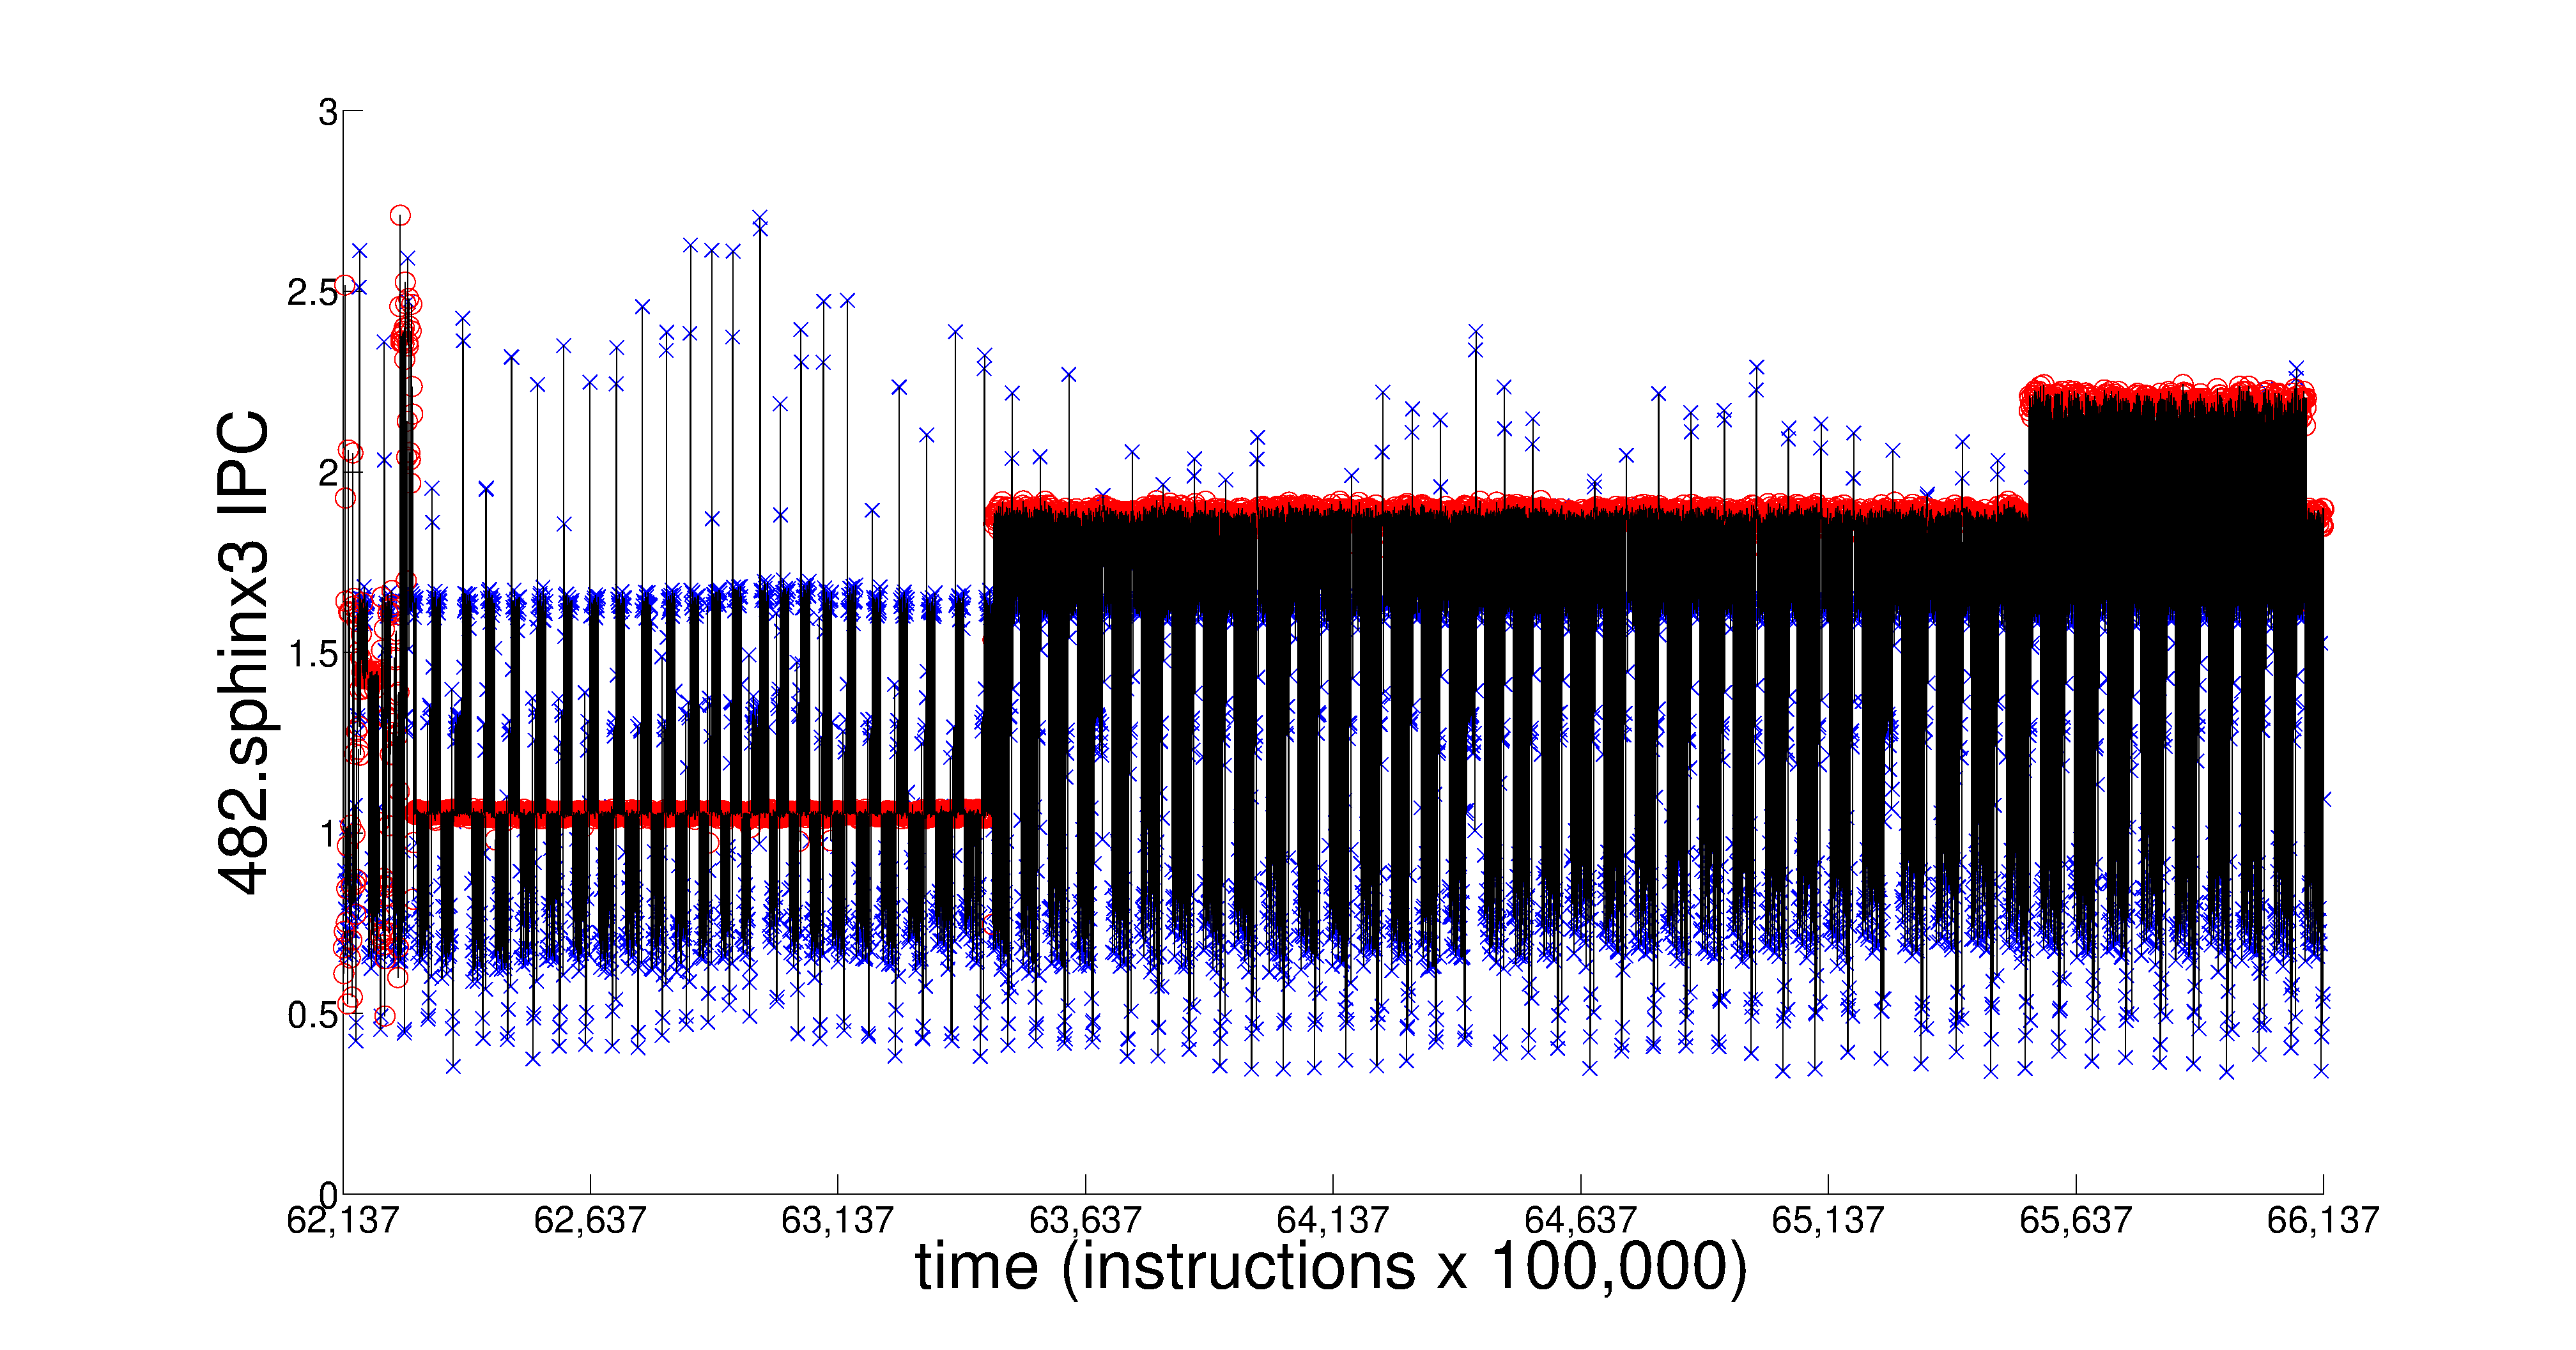
\includegraphics[width=0.5\textwidth]{figs/sphinxPredicTS}
     \caption{An LMA-based forecast of the last 4,000 points of a
       processor-load performance trace from the {\tt 482.sphinx3}
       benchmark.  Red circles and blue $\times$s are the true and
       predicted values, respectively; vertical bars show where these
       values differ.}
\label{fig:predsphinx}
\end{figure}

Table~\ref{tab:PredError} presents detailed results about the
prediction accuracy of this algorithm on four different examples: the
{\tt col\_major} and {\tt 482.sphinx3} programs in
Figures~\ref{fig:cachePredTS} and~\ref{fig:predsphinx}, as well as
another simple microkernel that initializes the same matrix as {\tt
  col\_major}, but in row-major order, and another complex program
({\tt 403.gcc}) from the SPEC cpu2006 benchmark suite.  Both
microkernels were run on the Intel Core
Duo\textsuperscript{\textregistered} machine; both SPEC benchmarks
were run on the Intel i7\textsuperscript{\textregistered} machine.  We
calculated a figure of merit for each prediction as follows.  We held
back the last $k$ elements\footnote{Several different prediction
  horizons were analyzed in our experiment; the results reported in
  this paper are for $k$=4000} of the $N$ points in each measured time
series, built the forecast model by embedding the first $N-k$ points,
used that embedding and the LMA method to predict the next $k$ points,
then computed the Root Mean Squared Error (RMSE) between the true and
predicted signals:
$$RMSE = \sqrt{\frac{\sum_{i=1}^k(c_i-\hat{p_i})^2}{k}}$$
%
To compare the success of predictions across signals with different
units, we normalized RMSE as follows:
$$nRMSE = \frac{RMSE}{X_{max,obs}-X_{min,obs}}$$
%
% The smaller the nRMSE, obviously, the more accurate the prediction.

  \begin{table}[htbp]
   % increase table row spacing, adjust to taste
   \renewcommand{\arraystretch}{1.3}
   \caption{Normalized root mean squared error (nRMSE) of 4000-point
     predictions of memory \& processor performance from different
     programs.}
   \label{tab:PredError}
   \centering
   % Some packages, such as MDW tools, offer better commands for making tables
   % than the plain LaTeX2e tabular which is used here.
%   \begin{tabular}{|c|c|c|c|c|c|}
%     \hline
%      & cache misses NRMSE & IPC NRMSE \\
%     \hline
%     \tt{row\_major}  & 0.0102  & 0.0095 \\
%          \hline
%     \tt{col\_major}  &0.0055& 0.0071 \\
%     \hline
%     \tt{403.gcc}  & 0.0865& 0.1805 \\
%          \hline
%     \tt{482.sphinx3} & 0.1142& 0.2946 \\
%      \hline
%   \end{tabular}
% \end{table}
   \begin{tabular}{|c|c|c|c|c|c|}
     \hline
      & cache miss rate & instrs per cycle \\
     \hline
     \tt{row\_major}  & 0.0324  & 0.0778 \\
          \hline
     \tt{col\_major}  &0.0080& 0.0161 \\
     \hline
     \tt{403.gcc}  & 0.1416& 0.2033 \\
          \hline
     \tt{482.sphinx3} & 0.2032& 0.3670 \\
      \hline
   \end{tabular}
 \end{table}

The results in Table~\ref{tab:PredError} show a clear distinction
between the two microkernels, whose future behavior can be
predicted effectively using this simple deterministic modeling
strategy, and the more-complex SPEC benchmarks, for which this
prediction strategy does not work nearly as well.
% Removed for space
% For both processor load (IPC) and memory usage (cache-miss rate),
% forecasts for {\tt 482.sphinx3} and {\tt 403.gcc} are much worse than
% for \verb|col_major| or \verb|row_major|.
%
This begs the question: If these traces all come from deterministic
systems---computers---then why are they not equally predictable?  Our
conjecture is that the sheer complexity of the dynamics of the SPEC
benchmarks running on the Intel i7\textsuperscript{\textregistered}
machine make them effectively impossible to predict.

%% [[If space: Add a segue sentence: next section uses permutation
%% entropy to explore that conjecture.]]

\section{Measuring Complexity}\label{sec:meaComplex}

For the purposes of this paper, one can view entropy as a measure of complexity
and predictability in a time series.  A high-entropy time series is almost
completely unpredictable---and conversely.  This can be made more rigorous:
Pesin's relation \cite{pesin77} states that in chaotic dynamical systems, the
Shannon entropy rate is equal to the sum of the positive Lyapunov exponents,
$\lambda_i$. The Lyapunov exponents directly quantify the rate at which nearby
states of the system will diverge with time: $\left| \Delta x(t) \right| \approx
e^{\lambda t} \left| \Delta x(0) \right|$.  The faster the divergence, the more
difficult prediction becomes.

Utilizing entropy as a measure of temporal complexity is by no means a new idea
\cite{Shannon1951, mantegna1994linguistic}.  Its effective usage requires
categorical data: $x_t \in \mathcal{S}$ for some finite or countably infinite
\emph{alphabet} $\mathcal{S}$, whereas data taken from real-world systems is
effectively real-valued.  To get around this, one must discretize the data---
typically achieved by binning.  Unfortunately, this is rarely a good solution to
the problem, as the binning of the values introduces an additional dynamic on
top of the intrinsic dynamics whose entropy is desired.  The field of symbolic
dynamics studies how to discretize a time series in such a way that the
intrinsic behavior is not perverted, but these methods are fragile in the face
of noise and require further understanding of the underlying system, which
defeats the purpose of measuring the entropy in the first place.

Bandt and Pompe introduced the \emph{permutation entropy} (PE) as a ``natural
complexity measure for time series" \cite{bandt2002per}.  Permutation entropy
employs a method of discretizing real-valued time series that follows the
intrinsic behavior of the system under examination.  Rather than looking at the
statistics of sequences of values, as is done when computing the Shannon
entropy, permutation entropy looks at the statistics of the \emph{orderings} of
sequences of values using ordinal analysis. Ordinal analysis of a time series is
the process of mapping successive time-ordered elements of a time series to
their value-ordered permutation of the same size.  By way of example, if $(x_1,
x_2, x_3) = (9, 1, 7)$ then its \emph{ordinal pattern}, $\phi(x_1, x_2, x_3)$,
is $231$ since $x_2 \leq x_3 \leq x_1$.  This method has many features; among
other things, it is generally robust to observational noise and requires no
knowledge of the underlying mechanisms.

\begin{mydef}[Permutation Entropy]

  Given a time series $\{x_t\}_{t = 1,\dots,T}$. Define $\mathcal{S}_n$ as all
  $n!$ permutations $\pi$ of order $n$. For each $\pi \in \mathcal{S}_n$ we
  determine the relative frequency of that permutation occurring in $\{x_t\}_{t
  = 1,\dots,T}$:
  \begin{align*}
    p(\pi) = \frac{\left|\{t|t \leq T-n,\phi(x_{t+1},\dots,x_{t+n}) = \pi\}\right|}{T-n+1}
  \end{align*}
  Where $|\cdot|$ is set cardinality. The \emph{permutation entropy} of order $n
  \ge 2$ is defined as
  \begin{align*}
  H(n) = - \sum_{\pi \in \mathcal{S}_n} p(\pi) \log_2 p(\pi)
  \end{align*}

\end{mydef}

Notice that $0\le H(n) \le \log_2(n!)$ \cite{bandt2002per}.  With this in mind,
it is common in the literature to normalize permutation entropy as follows:
$\frac{H(n)}{\log_2(n!)}$.  With this convention, ``low'' entropy is close to 0
and ``high'' entropy is close to 1. Finally, it should be noted that the
permutation entropy has been shown to be identical to the Shannon entropy for
many large classes of systems \cite{amigo2012permutation}.

Here we will be utilizing a variation of the permutation entropy, the
\emph{weighted permutation entropy} (WPE)~\cite{fadlallah2013}. The weighted
permutation entropy attempts to correct for observational noise which is larger
than some trends in the data, but smaller than the larger scale features --- for
example, a signal that switches between two fixed points with noise about those
fixed points. The weighted permutation entropy would be dominated by the
switching rather than by the stochastic fluctuation. To accomplish this, the
\emph{weight} of a permutation is taken into account:
\begin{align*}
  w(x_{t+1:t+n}) = \frac{1}{n}
                 \sum_{x_i \in \{x_{t+1:t+n}\}}
                 \left( x_i - \bar{x}_{t+1:t+n} \right)^2
\end{align*}
where $x_{t+1:t+n}$ is a sequence of values $x_{t+1}, \ldots, x_{t+n}$, and
$\bar{x}_{t+1:t+n}$ is the arithmetic mean of those values.

The weighted probability of a permutation is then:
\begin{align*}
  p_w(\pi) = \frac{\displaystyle \sum_{t \le T - n} w(x_{t+1:t+n}) \cdot \delta(\phi(x_{t:t+n}), \pi) }{\displaystyle \sum_{t \le T - n} w(x_{t+1:t+n})}
\end{align*}
where $\delta(x, y)$ is 1 if $x = y$ and 0 otherwise. Effectively, this weighted
probability enhances permutations involved in ``large'' features and demotes
permutations which are small in amplitude relative to the features of the time
series. The weighted permutation entropy is then:
\begin{align*}
  H_w(n) = - \sum_{\pi \in \mathcal{S}_n} p_w(\pi) \log_2 p_w(\pi)
\end{align*}

In practice, calculating permutation entropy and weighted permutation entropy
involves choosing a good value for the word length $n$. The primary
consideration is that the value be large enough that forbidden ordinals are
discovered, yet small enough that reasonable statistics over the ordinals are
gathered: e.g.:
\begin{align*}
n = \operatornamewithlimits{argmax}_\ell \{ T \gtrapprox 100 \ell! \},
\end{align*}
assuming an average of 100 counts per ordinal is sufficient. In the literature,
$3 \le n \le 6$ is a standard choice --- generally without any formal
justification. In theory, the permutation entropy should reach an asymptote with
increasing $n$, but that requires an arbitrarily long time series. In practice,
what one should do is calculate the \emph{persistent} permutation entropy by
increasing $n$ until the result converges, but data length issues can intrude
before that convergence is reached.


% Table~\ref{tab:pe} shows the permutation entropy results for the
% examples considered in this paper, with the nRMSPE prediction
% accuracies from the previous section included alongside for easy
% comparison.
%
% \begin{table}[htbp]
%   % increase table row spacing, adjust to taste
%   \renewcommand{\arraystretch}{1.3}
%   \caption{TCM NRMSE and PE NORMS}
%   \label{tab:table_example}
%   \centering
   % Some packages, such as MDW tools, offer better commands for making tables
   % than the plain LaTeX2e tabular which is used here.
%   \begin{tabular}{|c|c|c|c|c|c|}
%     \hline
%     TCM & NRMSE & $m=3$  &$m=4$&$m=5$&$m=6$\\
%     \hline
%     \tt{row\_major} & 0.0102 & 0.7900  &0.6751&0.5458&0.4491\\
%     \hline
%     \tt{col\_major} & 0.0055 & 0.6411  &0.5029&0.4515&0.3955 \\
%     \hline
%     \tt{403.gcc} & 0.0865 & 0.9954  &0.9916&0.9880&0.9835\\
%     \hline
%     \tt{482.sphinx3} & 0.1142 & 0.9958  &0.9913&0.9866&0.9802 \\
%      \hline
%   \end{tabular}
% \end{table}
%
%%  \begin{table}[htbp]
%%   % increase table row spacing, adjust to taste
%%   %\renewcommand{\arraystretch}{1.3}
%%   \caption{Cache-miss rate performance traces: prediction error
%%     (nRMSPE) and permutation entropy}
%%   \label{tab:TCMpe}
%%   \centering
%%   % Some packages, such as MDW tools, offer better commands for making tables
%%   % than the plain LaTeX2e tabular which is used here.
%%   \begin{tabular}{|c|c|c|c|c|c|}
%%     \hline
%%      & nRMSE   &$n=4$&$n=5$&$n=6$\\
%%     \hline
%%     \tt{row\_major}  & 0.0324  &0.6751&0.5458&0.4491\\
%%     \hline
%%     \tt{col\_major}  & 0.0080  &0.5029&0.4515&0.3955 \\
%%     \hline
%%     \tt{403.gcc}  & 0.1416  &0.9916&0.9880&0.9835\\
%%     \hline
%%     \tt{482.sphinx3}  & 0.2032  &0.9913&0.9866&0.9802 \\
%%      \hline
%%   \end{tabular}
%% \end{table}
%
% \begin{table}[htbp]
%   % increase table row spacing, adjust to taste
%   \renewcommand{\arraystretch}{1.3}
%   \caption{IPC NRMSE and PE NORMS}
%   \label{tab:table_example}
%   \centering
%   % Some packages, such as MDW tools, offer better commands for making tables
%   % than the plain LaTeX2e tabular which is used here.
%   \begin{tabular}{|c|c|c|c|c|c|}
%     \hline
%     ipc & NRMSE & $n=3$  &$n=4$&$n=5$&$n=6$\\
%     \hline
%      \tt{row\_major} & 0.0095 & 0.9912  &0.9723&0.9354&0.8876\\
%     \hline
%      \tt{col\_major} & 0.0071 & 0.9428  &0.8356&0.7601&0.6880\\
%     \hline
%     \tt{403.gcc} & 0.1805 & 0.9918  &0.9862&0.9814&0.9764\\
%     \hline
%     \tt{482.sphinx3} & 0.2946 & 0.9978  &0.9951&0.9914&0.9849 \\
%      \hline
%   \end{tabular}
% \end{table}
%
%%  \begin{table}[htbp]
%%   % increase table row spacing, adjust to taste
%%   %\renewcommand{\arraystretch}{1.1}
%%   \caption{Processor load performance traces: prediction error
%%     (nRMSPE) and permutation entropy}
%%   \label{tab:IPCpe}
%%   \centering
%%   % Some packages, such as MDW tools, offer better commands for making tables
%%   % than the plain LaTeX2e tabular which is used here.
%%   \begin{tabular}{|c|c|c|c|c|}
%%     \hline
%%      & nRMSPE   &$n=4$&$n=5$&$n=6$\\
%%     \hline
%%      \tt{row\_major} & 0.0778  &0.9723&0.9354&0.8876\\
%%     \hline
%%      \tt{col\_major} & 0.0161   &0.8356&0.7601&0.6880\\
%%     \hline
%%     \tt{403.gcc} & 0.2033   &0.9862&0.9814&0.9764\\
%%     \hline
%%     \tt{482.sphinx3} & 0.3670 & 0.9951&0.9914&0.9849 \\
%%      \hline
%%   \end{tabular}
%% \end{table}
%
 %  \begin{table}[htbp]
 %   \caption{Prediction error (in nRMSPE) and permutation entropy (for
 %     different wordlengths $n$}
 %   \label{tab:pe}
 %   \centering
 %   \begin{tabular}{|c|c|c|c|c|c|}
 %     \hline
 %      {\bf cache misses} & error   &$n=4$&$n=5$&$n=6$\\
 %     \hline
 %     \tt{row\_major}  & 0.0324  &0.6751&0.5458&0.4491\\
 %     \hline
 %     \tt{col\_major}  & 0.0080  &0.5029&0.4515&0.3955 \\
 %     \hline
 %     \tt{403.gcc}  & 0.1416  &0.9916&0.9880&0.9835\\
 %     \hline
 %     \tt{482.sphinx3}  & 0.2032  &0.9913&0.9866&0.9802 \\
 %      \hline
 %      \hline
 %      {\bf insts per cyc} & error   &$n=4$&$n=5$&$n=6$\\
 %     \hline
 %      \tt{row\_major} & 0.0778  &0.9723&0.9354&0.8876\\
 %     \hline
 %      \tt{col\_major} & 0.0161   &0.8356&0.7601&0.6880\\
 %     \hline
 %     \tt{403.gcc} & 0.2033   &0.9862&0.9814&0.9764\\
 %     \hline
 %     \tt{482.sphinx3} & 0.3670 & 0.9951&0.9914&0.9849 \\
 %      \hline
 %   \end{tabular}
 % \end{table}

The relationship between prediction accuracy and the permutation
entropy (PE) is as we conjectured: performance traces with high
PE---those whose temporal complexity is high, in the sense that little
information is being propagated forward in time---are indeed harder to
predict using the simple deterministic forecast model described in the
previous section.  The effects of changing $n$ are also interesting:
using a longer wordlength generally lowers the PE---a natural
consequence of finite-length data---but the falloff is less rapid in
some traces than in others, suggesting that those values are closer to
the theoretical asymptote that exists for perfect data.  The
persistent PE values of 0.5--0.6 for the {\tt row\_major} and {\tt
  col\_major} cache-miss traces are consistent with dynamical chaos,
further corroborating the results of~\cite{mytkowicz09}.  (PE values
above 0.97 are consistent with white noise.)  Interestingly, the
processor-load traces for these two microkernels exhibit more temporal
complexity than the cache-miss traces.  This may be a consequence of
the lower baseline value of this time series.

% In Table~\ref{tab:TCMpe} \& \ref{tab:IPCpe} the behavior of the PEs as
% they limit to their asymptotic values is observed. A feature of note
% is that some of the signals drop off and some do not.  For example at
% $m=4$ {\tt col\_major} is at 0.8356, a fairly high entropy, however as
% $m$ is increased to 6 the PE plummets to 0.6880: a value consistent
% with a chaotic time series. Notice this also corresponds to a very low
% nRMSE. In contrast, consider the permutation entropy of the processor
% load of {\tt 482.sphinx3}: with $m=4$ it is 0.9951 and only drops to
% 0.9849 at $m=6$. This is consistent with the signal also having the
% highest nRMSE.

\section{ Conclusions \& Future Work}\label{sec:conc}

The results presented here suggest that permutation entropy---a
ordinal calculation of forward information transfer in a time
series---is an effective metric for predictability of computer
performance traces. Experimentally, traces with a persistent PE
$\gtrapprox 0.97$ have a natural level of complexity that may
overshadow the inherent determinism in the system dynamics, whereas
traces with PE $\lessapprox 0.7$ seem to be highly predictable (viz.,
at least an order of magnitude improvement in nRMSPE).

If information is the limit, then gathering and using more information
is an obvious next step.  There is an equally obvious tension here
between data length and prediction speed: a forecast that requires
half a second to compute is not useful for the purposes of real-time
control of a computer system with a MHz clock rate.  Another
alternative is to sample several system variables simultaneously and
build multivariate delay-coordinate embeddings.  Existing approaches
to that are computationally prohibitive
\cite{cao-multivariate-embedding}.  We are working on alternative
methods that sidestep that complexity.

%%This use of permutaiotn entropy is a useful application of information
%%theory to computer performance modeling because it gives you a simple
%%and fast way to decide whether building a model and trying to forecast
%%the future is worthwhile or if guessing the mean is just as effective.
%%End with a sentence tying back to power management and world peace.


%\begin{it}
%Summarize the results.

%Paragraphs on the issues that come up, including one about the "amount
%of info" one: if one could sample more variables, for instance, one
%might be able to do a better job of predicting more-complex traces.
%Segue to some handwaving about multivariable LMA models; tie this back
%to the "computers are NLD systems" stuff in the intro.  This is a real
%challenge; current approaches to this modelling problem have the major
%issue of taking way too long to build.  And that's a big issue if
%you're trying not just to classify, but to predict.  In a system that
%runs at MHz speeds, a prediction that takes milliseconds to compute is
%not useful.
%\end{it}




%[[Joshua: It may be interesting to look at the PE as a function of
%prediction horizon. It is known to me that certain start and end
%locations in the prediction strategy result in different prediction
%accuracy. Is it the case that when the algorithm tanks it is also the
%case that PE of the **TEST**(the 10\% we cut off )is high? This may
%be a great way to illustrate the concept if it works... OR maybe do
%complexity of forward path in embedding space?]]  some notes about
%this looking at row Cache 1000 very good RMSPE 21.4167 m = 3 4 5 6
%1.4192 2.1286 2.5942 2.9230 row Cache 2000 very good RMSPE 19.0990 m
%= 3 4 5 6 1.4145 2.1305 2.5825 2.9095 so even better row Cache 2010
%RMSPE 19.9716 m = 3 4 5 6 1.4149 2.1311 2.5830 2.9096 row Cache 1990
%RMSPE 19.1465 So prediction Horizons ranked in order of best RMSPE
%RMSPE L 3 4 5 6 1st 19.0990 2000 1.4145 2.1305 2.5825 2.9095 2nd
%19.1465 1990 1.4151 2.1293 2.5803 2.9067 3rd 19.9716 2010 1.4149
%2.1311 2.5830 2.9096 3rd 21.4167 1000 1.4192 2.1286 2.5942 2.9230
%ipcgcc m = 3 pe = 1.7770 penorm = 0.9918 m= 4 pe = 3.1341 penorm =
%0.9862 m = 5 pe = 4.6985 penorm = 0.9814 m=6 pe = 6.4242 penorm =
%0.9764 m=7 pe = 8.2450 penorm = 0.9671 >> [pe penorm] =
%permCalc(gcc100TCM,5,1) pe = 4.7299 penorm = 0.9880 >> [pe penorm] =
%permCalc(gcc100TCM,6,1) pe = 6.4707 penorm = 0.9835



%****BEYOND THIS POINT IS A DIFFERNT PAPER*** JOSHUA WILL CLEAN THIS OUT, JUST HERE FOR REFERNCE****
%\section{Introduction: What is Permutation Entropy}


%%\begin{it}
%%Here I want to talk about the definition and algorithm for computing it. Maybe briefly talk about the asymptotic %properties. (i.e., same as metric topological in limit. Converges to dominate leap if not normalized etc. )
%%\end{it}
%
%When analyzing a time series there are several standard characterizations of complexity, including (but not limited to) entropy, Lyapunov exponents and fractal dimensions. Rigorous definitions of all these quantities exist if the observation is a \emph{noise-free} trajectory of a \emph{single} dynamical system. To an experimental-time-series analyst these are luxuries that are rarely (if ever) realized. Many times experimental observation have noise involved such as sensor error, or very commonly in the computer world finite-precision error.
%
%Unfortunately the standard algorithms for calculating many of these complexity measures are highly sensitive to noise and give spurious results in the presence of noisy observations. Even worse, if a time-series observation measures multiple dynamical systems or dynamical systems that undergo bifurcations\footnote{A drastic change in the behavior of the dynamical system, generally associated with parameter drift.} then all of the standard algorithms for estimating complexity, (e.g., correlation dimension) go out the window. Bandt and Pompe first introduced \emph{permutation entropy} as a ``natural complexity measure for time series" in 2002 \cite{bandt2002per}.
%
%
%As explained in \cite{bandt2002per}, permutation entropy is a simple complexity measure that is easily calculated for any time series, be it stochastic, periodic, quasi-periodic, chaotic, noisy or any combination of these. Most importantly for analysis of computer performance, permutation entropy as defined in \cite{bandt2002per} yields meaningful results even if observational or dynamical noise is present \cite{bandt2002per}.
%
%
%
%
%Analyzing entropies as  a complexity measure is not a new concept, however the way that the entropy is estimated in \cite{bandt2002per} is novel and particularly useful when little is known about the underlying process.   As discussed in \cite{bandt2002per}, the standard entropy one considers is Shannon entropy.
%
%
%As a quick review of Shannon entropy, we follow the treatment in \cite{amigo2012permutation}. Given a finite alphabet $\mathcal{S} = \{s_1,....,s_{|\mathcal{S}|}\}$, define an information source as a discrete-time, stationary stochastic process $X = \{X_n\}_{n \in \mathbb{N}_0}$ where $X_n$ are random variables on a common probability space taking on values from $\mathcal{S}$. A realization of $X$ is a one-sided sequence $x_0^{\infty} = (x_n)_{n \in \mathbb{N}_0}$ called a \emph{message}. The elements $x_n$ of $\mathcal{S}$ are the \emph{symbols}(a.k.a letters) of the language. A finite segment of the message, say $x_k^{k+m-1} = x_kx_{k+1} \dots x_{k+m-1}$ is called a \emph{word} (of length m). We then define $p(x_0^{m-1})$ to be the probability of the word $x_0^{m-1}$ to appear some where in the message. The shannon entropy of the data source $X$ is defined as: \begin{equation}\label{eq:shannonentropy}
%h(X) = - \lim_{m\to\infty}\frac{1}{m}\sum p(x_0^{m-1})\log p(x_0^{m-1})
%\end{equation}
%
%For the purposes of this paper once can view entropy as a measure of complexity and predictability in a time series. A high entropy almost completely unpredictable and a small entropy is completely predictable. This spectrum is outlined very nicely in \cite{amigo2012permutation}: ``Periodic or quasiperiodic sequences have vanishing or negligible complexity. At the opposite end, independent and identically distributed random sequences (white noise) have asymptotically divergent permutation entropies, owing to the fact that the number of allowed (or ``admissibleÓ) ordinal patterns grows superexponentially with length. Between both ends lie the kind of sequences we are interested in."
%
%This illustrates why utilizing entropy as a measure for complexity is, in theory, a great candidate. There are several fundamental drawbacks with this approach when analyzing real-world time series. The two most fundamental problems are as follows:
%
%\begin{enumerate}
%\item Elements of an experimental time series $x_t \in \mathbb{R}$ which implies $x_t \notin \mathcal{S}$, for a finite alphabet $\mathcal{S}$.
%\item Time series are always finite in length so the limit in \ref{eq:shannonentropy} never exists in practice.
%\end{enumerate}
%
%
%The common practice to address item 1 is to perform \emph{symbolization} on the time series you want to analyze. Symbolization is the process of defining a dynamic preserving map $\phi: \mathbb{R}^m \to \mathcal{S}$, i.e., for each $x_t$ (or block $x_k^{k+m-1} = x_kx_{k+1} \dots x_{k+m-1}$) we must assign a symbol from $\mathcal{S}$ in such a way that the time series has the same fundamental properties.  There are several approaches to symbolization, the standard approach is partitioning. Assume, $x_t$ has the capability of taking on infinitely many values, defining the space $X$ to be the space where these $x_t$ are drawn. We then define a partition on this space $X = P_1 \cup...\cup P_m$, and define $\mathcal{S} = \{1,\dots,m\}$. Then $\phi(x_t) = i$ if $x_t \in P_i$. We can then calculate the Shannon entropy of the transformed time series, which in the limit of $m$ converges to the Kolmogorov-Sinai entropy \cite{bandt2002per}. This approach to symbolization is computationally infeasable as we need an infinite number of partitions of an infinite time series. For \emph{extremely} rare cases, there exists a \emph{generating} partition where this limit is not necessary. However, finding such a partition even for a simple two-dimensional map like Henon is non-trivial \cite{bandt2002per}. Finding a generating partition for an arbitrary time series is for all intensive purposes impossible.
%
%[[[Maybe also talk about Mischaikow's approach to this with isolating neighborhoods and homology...but might be off topic. ]]]
%
%
%.....
%
%
%
%Instead of this approach to symbolization, Bandt et al. take the approach that ``the symbol sequence must come naturally for the time series, without any further model assumptions" \cite{bandt2002per}. To do this they perform symbolization through ordinal analysis. Ordinal analysis of a time series is the process of mapping the ordered successive elements of a time series to a permutation of the same size based on their original time-based ordering.[[Need a better way of wording this]]. This is also referred to in the literature as the permutation complexity \cite{amigo2012permutation}  For example, if $(x_1,x_2,x_3) = (9,1,7)$ then $\phi$ maps $(x_1,x_2,x_3)$ to the permutation $231$ since $x_2 < x_3<x_1$. A great explanation of why this is an interesting symbolization is found in \cite{amigo2012permutation} :
%
%\begin{quote}The study of permutation complexity, which we call ordinal analysis, can be envisioned as a new kind of symbolic dynamics whose basic blocks are ordinal patterns. Interesting enough, it turns out that under some mild mathematical assumptions, not all ordinal patterns can be materialized by the orbits of a given one- or multi-dimensional deterministic dynamics, not even if this dynamic is chaoticÑ contrarily to what happens with the symbol patterns. As a result, the existence of ÒforbiddenÓ (i.e., not occurring) ordinal patterns is always a persistent dynamical feature, in opposition to properties such as proximity and correlation which die out with time in a chaotic dynamic. Moreover, if an ordinal pattern is forbidden, its absence pervades all longer patterns in form of more missing ordinal patterns, called outgrowth forbidden patterns. Admissible ordinal patterns grow exponentially with length, while forbidden patterns do superexponentially. Since random (unconstrained) dynamics has no forbidden patterns with probability 1, their existence can be used as a fingerprint of deterministic orbit generation.
%\end{quote} Essentially by analyzing the permutation entropy of a time series we are gaining information as to the complexity of the system without any other information available, whether the time series is generated by a random process or the trajectory of a deterministic dynamical system. Now that we have justified why the study of permutation entropy is interesting let us define it. For this we follow \cite{bandt2002per}.
%
%
%\begin{mydef}[Permutation Entropy]
%Given a time series $\{x_t\}_{t = 1,\dots,T}$. Define $\mathcal{S}_n$ as all $n!$ permutations $\pi$ of order $n$. For each $\pi \in \mathcal{S}_n$ we determine the relative frequency of that permutation occurring in $\{x_t\}_{t = 1,\dots,T}$: \begin{equation}\label{eq:permprob}
%p(\pi) = \frac{|\{t|t\le T-n,\phi(x_{t+1},\dots,x_{t+n}) = \pi\}|}{T-n+1}\end{equation}
%Where $|\cdot|$ is set cardinality. The \emph{permutation entropy} of order $n\ge 2$ is defined as $$H(n) = - \sum_{\pi \in \mathcal{S}_n} p(\pi)\log_2p(\pi)$$ Notice that $0\le H(n) \le \log_2(n!)$,\cite{bandt2002per}. With this in mind, it is common in the literature to present permutation entropy normalized, i.e., $\frac{H(n)}{\log_2(n!)}$. With this convention, \emph{low} entropy is close to 0 and \emph{high} entropy is entropy close to 1.
%\end{mydef}
%
%Notes: According to \cite{bandt2002per} equation (\ref{eq:permprob}) estimates the frequency of $\pi$ as good as possible for a finite series of values. To determine $p(\pi)$ exactly, we have to assume an infinite time series and take the limit as $T\to \infty$ in (\ref{eq:permprob}). Bandt et al., also point out that this limit exists under a very weak stationarity condition: for $k\le n$, the probability for $x_t<x_{t+k}$ should not depend on $t$.
%
%It should also be noted that this is discrete-metric (or shannon) permutation entropy, to be distinguished from topological permutation entropy (a.k.a. permutation capacity). Topological permutation entropy is defined in \cite{amigo2012permutation} as: $$h(\{x_t\}_{t = 1,\dots,\infty}) =  \lim_{L\to\infty}\frac{1}{L}logN(L)$$ where $N(L)$ is the number of distinct ordinal patterns that occur of order $L$. This is a measure of how many distinct permutations of length $L$ are realized as opposed to counting the frequency at which each occurs as is the case in metric permutation entropy \cite{amigo2012permutation}. It can be shown that metric and topological entropy both converge to the true value with probability 1 in the limit.  (citation for this). When we say permutation entropy in this paper we are referring to that defined in \ref{eq:permprob}.
%
%\section{Detecting changes in a time series}
%
%Permutation entropy is a measure of the complexity of time series as a whole, but it can also be used to calculate a dynamical shift in a time series as illustrated in \cite{cao2004det}. To detect dynamical changes in a time series we follow the methods of \cite{cao2004det}. Partition the time series  $\{x_t\}_{t = 1,\dots,T}$ into overlapping\footnote{Following \cite{cao2004det} we use maximal overlapping block. (A window shift of 1.)} (or nonoverlapping) blocks. Calculate $H(n)$ for each block, and treat $H(n)$ as a function of time.  According to \cite{cao2004det} drastic changes in permutation entropy can indicate change in the underlying model.
%
%In addition to introducing this block method, \cite{cao2004det} introduce the use of a \emph{lag} when calculating permutation entropy. This is identical to the lag used in delay coordinate embedding and often the same language is used. Cao et al. describe the process of symbolization in \cite{bandt2002per} as embedding the time series in an $m$ dimensional symbol space. When we symbolize a scalar time series,$\{x_t\}_{t = 1,\dots,T}$, we first embed the scalar time series into $m$ dimensional vectors before matching this to a symbol in $\mathcal{S}_m$. So pre-symbolization our time series changes from scalar to objects of the form:  $$[x(i),\,x(i+1),\,\dots,x(i+(m-1)]$$ This vector is then mapped by $\phi$ to a symbol in $\mathcal{S}_m$. Cao et al. argue that we can view this as embedding the time series in an $m$ dimensional space with lag 1. Cao et al. then state ``Since in practice the optimal $L$[lag] may be different from 1, we shall present the idea for any $m$[embedding dimension] and $L$."\footnote{No further explanation is given about why this is the case.} To not confuse notation we define $\tau$ to be the lag parameter. The process of symbolization then starts with transforming the scalar time series into a set of vectors of the form $$[x(i),\,x(i+\tau),\,\dots,x(i+(m-1)\tau]$$ where $\tau\ge1$.
%
%\subsection{Example: Concatenated Time Series}\label{sec:concatenate}
%As an example of this detection, consider Figure \ref{fig:ts-banded} (a). This is a plot of a concatenated time series comprised of several orbits of the Logistic map with varying parameters as well as intermittent noise. Each concatenated band (either an orbit of the Logistic map or noise) is 50,000 points. The bands of noise are generated with Matlab's \verb|randsample|, using the chaotic bands as the sampling population. Each Logistic map trajectory begins at $x=0.6$. The period-two trajectories have an $R$ of 3.2, the period-three trajectory has an R of 3.838, and the chaotic trajectories have an $R$ of 3.65.
%
%The concatenated time series is comprised of two period-two trajectories($t=0-50,000$ and $t=250,000-300,000$), one period-three trajectory($t=100,000-150,000$), two chaotic trajectories ($t=50,000-100,000$ and $t=200,000-250,000$, and two different bands of noise($t=150,000-200,000$ and $t=300,000-350,000$). Visually the bands of noise and the chaotic trajectory are indistinguishable. If this were an observed time series from a real process, it would be impossible to visually identify which bands were generated deterministically and which were simply noise. If we calculate block permutation entropy as discussed in \cite{cao2004det} and plot this as a function of time it becomes very clear which bands have structure and which do not.
%
%In Figure \ref{fig:ts-banded} (b) we plot the concatenated time series, as well as permutation entropy as a function of time(red, blue and green curves). The red, blue and green curves are the permutation entropy calculated using $m=5$ and $\tau = 1,2,3$ (respectively). Using these curves it is clear that bands 2 and 5 ($t=50,000-100,000$ and $t=200,000-250,000$) are chaotic because they have structure\footnote{Permutation entropy less than one.}. On the other hand, bands 4 and 7 ($t=150,000-200,000$ and $t=300,000-350,000$) have no structure\footnote{Permutation entropy of one.} and are the noise bands. This is in fact the case when comparing to the way the time series was constructed.
%
%The main advantage we can see to the use of lags other than 1 is for analysis of periodicity. This is also the major advantage listed in \cite{cao2004det}. Notice in the period 2 bands the blue curve (permutation entropy calculated with a lag of 2) is zero. This means that with a lag of 2 the period 2 orbit is perfectly structured\footnote{Equivalently, not enough permutations are being realized to impact the calculation of $H(n)$}. If we increase the lag to 3 (the green curve) the two period-two bands have a little bit of structure(as some permutations will be realized) but the period 3 band has zero permutation entropy.
%
%%TSLogistic = [period2Logistic;chaosLogistic;period3Logistic;randomSampleFromMap2;chaosLogistic;period2Logistic;randomSampleFromMap3];
%
%\begin{figure}
%  \centering
%  \subfigure{\includegraphics[width=\columnwidth]{figs/ts-banded-alone}}
%    {(a)}
%
%  \subfigure{\includegraphics[width=\columnwidth]{figs/ts-banded-pe}}
%  {(b)}
%  \caption{ (a) The concatenated time series discussed in Section~\ref{sec:concatenate}. (b) Plot of the concatenated time series from Section~\ref{sec:concatenate}, as well as permutation entropy as a function of time(blue,green and red curves). Each permutation entropy curve shown is calculated using $m=5$, however, the red,blue and green curve use a $\tau = 1,2,3$ respectively.}\label{fig:ts-banded}
%\end{figure}
%
%
%
%
%
%
%and what is it good for with forward pointer to the other sections
%
%
%
%\subsection{Example: The transient Logistic map}
%In Section~\ref{sec:concatenate} we discussed a time series which stayed in a parameter regime for long amounts of time and then abruptly changed. As we showed, permutation was a great proxy to detect this change. Another type of parameter change that may occur in a physical system is constant parameter drift, i.e., some parameter slowly changes over time. To explore this type of parameter drift we construct the same time series as was used in \cite{cao2004det}. Iterate the logistic map, starting with $R=2.8$, then at every iteration increase $R$ by $10^{-5}$ until $R=4$. The time series, which can be seen in Figure~\ref{fig:translogistic} appears very similar to the standard bifurcation diagram for the Logistic map. The curves in red and blue are the permutation entropy calculated with $m=5$ and $\tau = 1,2$ (respectively).
%
% As we can see, as bifurcations occur in the dynamics the permutation entropy changes as well. An interesting feature of block calculations are the spikes that occur at bifurcation points. As the block begins to encompass multiple regimes, e.g., fixed point and  period two, permutations are being realized for both regimes. This overlap causes an increase in the time series complexity, and thus a spike in the permutation entropy. The dips you see in the second half correspond to bands of periodicity which occur between the chaos. It is worth noting, that the blue curve (permutation entropy with lag 2) does not go to zero in the period 2 parameter range. This is because this is not a true period 2 orbit but transient that is moving across \emph{several} period 2 orbits, thus it maintains a higher level of complexity, albeit still very low.
%
% This illustrates that permutation entropy can not only distinguish between instant (and drastic) parameter shifts but also very slow and gradual parameter drift.
%
%\begin{figure}[ht]
%  \centering
%  \includegraphics[width=\columnwidth]{figs/tstranslog-perm}
%  \caption{Transient Logistic map time series and permutation entropy curves. Both permutation entropy curves are calculated with $m=5$, the red and blue correspond to $\tau = 1,2$ respectively.}
%  \label{fig:translogistic}
%\end{figure}
%%\begin{enumerate}
%%\item do with henon bifurcation. what happens near the broken chaotic window
%
%%\end{enumerate}
%
%
%\section{Possible Applications to Computer Systems Performance}
%
%
%\begin{enumerate}
%\item In this section I want to discuss the symbolization of performance traces and why this is advantageous over generating partitions and similar approaches.
%\item No model is assumed, some traces do appear to be stochastic some appear to be deterministic this provides ``proof" thereof. albeit not mathematical proof but CS proof for sure.
%\item We have essentially infinite data. So limits like $m!$ where $m$ is word length isn't really an issue for us.
%\end{enumerate}
%
%
%\subsection{Predictability and model change detection}
%
%Talk about how some explanatory models may be spinning their wheels because no transferable information. That is if you are introducing pure entropy at every time step really no use in using past values and statistically the mean is the most accurate.
%
%\begin{enumerate}
%\item Comp Performance goes under constant bifurcations. This allows autonomous detection of when a model is no longer valid. (need to be careful here with use of valid as to not be confused with model validation.
%\item Maybe can tell us if we should use a linear-stochastic, nonlinear-deterministic model or just guess the mean
%\end{enumerate}
%
%
%\begin{figure}[ht]
%  \centering
%  \includegraphics[width=\columnwidth]{figs/ts-rowcol-pe}
%  \caption{A time series of cache misses during the execution of the row-col microkernel. The red and blue curves are permutation entropy calculated using $\tau =1$ and $m=5,6$ (respectively). }\label{fig:rowcol}
%\end{figure}
%
%
%\begin{figure}[ht]
%  \centering
%  \includegraphics[width=\columnwidth]{figs/ts-gcc-pe}
%  \caption{A time series of instructions per cycle for the gcc spec benchmark. The red and blue curves are permutation entropy calculated using $\tau =1$ and $m=3,4$ (respectively). The lack of structure in such a signal illustrates that the use of deterministic models is most likely not the most advantageous.}\label{fig:gcc}
%\end{figure}
%
%
%
%\section{Pro and Cons}
%\subsection{Advantages of Permutation Entropy}
%Permutation entropy allows for symbolization of a time series without any further assumptions being made about the underlying system. In fact, virtually nothing needs to be known before applying this techniques. Other methods of symbolization require expert knowledge of the underlying system, such as generating partitions. These techniques have been applied to small data sets, this is truly an advantage especially when dealing with a lot of biological systems whose large datasets can be in the tens of thousands. The algorithm for computing permutation entropy is very straight forward and easy to explain. The actual code takes longer than I would like to run, but this seems to be an issue with my implementation and not the algorithm, as others state they have exceptionally fast algorithms. Although none of these algorithms are ever provided in the literature. The major advantages of permutation entropy is that it can quickly give us a rough estimate of where drastic changes in the time series which may have implications in model selection techniques. Permutation entropy also can give you a quick idea about if a system has deterministic structure. This has direct implications on what prediction strategies to implement.
%%\begin{enumerate}
%%\item Allows for symbolization without a model. Really emphasize we can obtain a symbolization without generating partitions which is the traditional approach here.
%%\item Small amounts of data not really a problem.
%%\item Maybe talk about how much data is needed per word length for results that mean anything.
%%\item Fairly easy to calculate, although need a more efficient method.
%%\item Gives a rough estimation of where drastic changes have occurred in a TS
%%\item Allows you to see if there is actually something predictable in the signal.
%%\end{enumerate}
%
%\subsection{Disadvantages of PE}
%There are three disadvantages with permutation entropy we can immediately see that need further thought to be overcome. The first is that it is sometimes hard to tell when a change in the dynamical system is not drastic enough to have a huge change on the entropy. For example, consider a dynamical system switching from a chaotic to a (different) chaotic regime. The permutation entropy may be very similar while the model is slightly different. Permutation entropy seems to be ill-suited for fine grain detection of this nature. Our current implementation is too slow for on-the-fly analysis. We do not believe this is an issue with permutation entropy itself but with our implementation. The literature all claims that fast algorithms exist.
%
%The biggest disadvantage for us in using permutation entropy is selection of parameters. To calculate permutation entropy, we have to choose an embedding dimension, a lag, and a block size. In all the literature we have found thus far, parameter selection is made based on persistence or matching the permutation entropy to known values. The problem comes when analyzing real time series these parameters seem to have a real impact on the results. Finding (or creating) a rigorous method for parameter selection is paramount in the use of this method for the analysis of real world time series.
%%\begin{enumerate}
%%\item Paramaters!
%%\item Currently numerically expensive although the literature disagrees. Think this might just be my implementation. Need to read the numerics section of the PE book.
%%\item Sometimes hard to tell a regime shift has occurred if the transition is chaotic to chaotic. or low period to low period.
%%\end{enumerate}

\section{New Figures and Tables}




\begin{table}[htdp]
\caption{ Embedding Parameters for reference if needed. }
\begin{center}
\begin{tabular}{|c|c|c|}
\hline
&$\tau$ & $m$ \\
\hline
gcc & 10& 13\\
col\_major  &2&12\\
SVD\_Full &  10  &  12 \\
SVD\_IPC\_Regime1 & 5 &14  \\
SVD\_IPC\_Regime2 & 10   &12  \\
SVD\_IPC\_Regime3 & 2   &9  \\
SVD\_IPC\_Regime4 &  3  & 11 \\
SVD\_IPC\_Regime5 &  23  & 10 \\
SVD\_IPC\_Regime6 &  30  & 12  \\
\hline
\end{tabular}
\end{center}
\label{default}
\end{table}%




\begin{table}[htdp]
\caption{Average nRMSE over 15 runs for each signal and average wpe at word length 5 and 6 for each signal. }
\begin{center}
\begin{tabular}{|c|c|c|c|c|c|}
\hline
                  & Horizon & nRMSE LMA           & nRMSE na\"{i}ve          & $l=5$                   & $l=6$                   \\
\hline
gcc               & 4,542   & $0.1407 \pm 0.0063$ & $0.1487 \pm 0.0066$ & $0.950991 \pm 0.001073$ & $0.942964 \pm 0.001256$ \\

col\_major        & 14,709  & $0.0252 \pm 0.0061$ & $0.1975 \pm 0.0436$ & $0.563640 \pm 0.003110$ & $0.513101 \pm 0.003365$ \\

%SVD\_Full         & 22,072  & $0.0323 \pm 0.0019$ & $0.1784 \pm 0.0040$ & $0.876517 \pm 0.004354$ & $0.850805 \pm 0.003454$ \\
SVD\_IPC\_Regime1 & 2,158   & $0.1680 \pm 0.0317$ & $0.3517 \pm 0.5223$ & $0.976109 \pm 0.008359$ & $0.957204 \pm 0.015623$ \\
SVD\_IPC\_Regime2 & 6,902   & $0.1716 \pm 0.0043$ & $0.1762 \pm 0.0012$ & $0.875984 \pm 0.005161$ & $0.846360 \pm 0.004420$ \\
SVD\_IPC\_Regime3 & 947     & $0.0507 \pm 0.0011$ & $0.5413 \pm 0.0005$ & $0.776841 \pm 0.007290$ & $0.715747 \pm 0.005605$ \\
SVD\_IPC\_Regime4 & 2,929   & $0.1288 \pm 0.0471$ & $0.2308 \pm 0.0867$ & $0.907348 \pm 0.008018$ & $0.824626 \pm 0.007707$ \\
SVD\_IPC\_Regime5 & 3,255   & $0.0235 \pm 0.0022$ & $0.1306 \pm 0.0003$ & $0.733272 \pm 0.007562$ & $0.677575 \pm 0.006792$ \\
SVD\_IPC\_Regime6 & 5,804   & $0.0196 \pm 0.0022$ & $0.0508 \pm 0.0003$ & $0.810087 \pm 0.013468$ & $0.747545 \pm 0.010607$ \\
\hline
\end{tabular}
\end{center}
\label{default}
\end{table}%




\begin{figure}
        \centering
        \begin{subfigure}{\textwidth}
                \includegraphics[width=\textwidth]{figs/svdipcfull}
                \caption{SVD IPC without coloring}
                \label{fig:gull}
        \end{subfigure}%
        \newline
        ~ %add desired spacing between images, e. g. ~, \quad, \qquad etc.
          %(or a blank line to force the subfigure onto a new line)
        \begin{subfigure}[b]{\textwidth}
                \includegraphics[width=\textwidth]{figs/svdipcregimescolored}
                \caption{SVD IPC with coloring}
                \label{fig:svdFullColored}
        \end{subfigure}
        ~ %add desired spacing between images, e. g. ~, \quad, \qquad etc.
          %(or a blank line to force the subfigure onto a new line)
         \caption{SVD Full Time Series }\label{fig:svdFull}
\end{figure}




\begin{figure}
        \centering
        \begin{subfigure}{\textwidth}
                \includegraphics[width=\textwidth]{figs/svdPrediction}
                \caption{SVD LMA Prediction}
                \label{fig:gull}
        \end{subfigure}%
        \newline
        ~ %add desired spacing between images, e. g. ~, \quad, \qquad etc.
          %(or a blank line to force the subfigure onto a new line)
        \begin{subfigure}[b]{\textwidth}
                \includegraphics[width=\textwidth]{figs/svdPredictionFull}
                \caption{SVD LMA Prediction with Full Time Series}
                \label{fig:svdFullColored}
        \end{subfigure}
        ~ %add desired spacing between images, e. g. ~, \quad, \qquad etc.
          %(or a blank line to force the subfigure onto a new line)
         \caption{SVD LMA Prediction Figures }\label{fig:svdFull}
\end{figure}



\begin{figure}
        \centering
        \begin{subfigure}{\textwidth}
                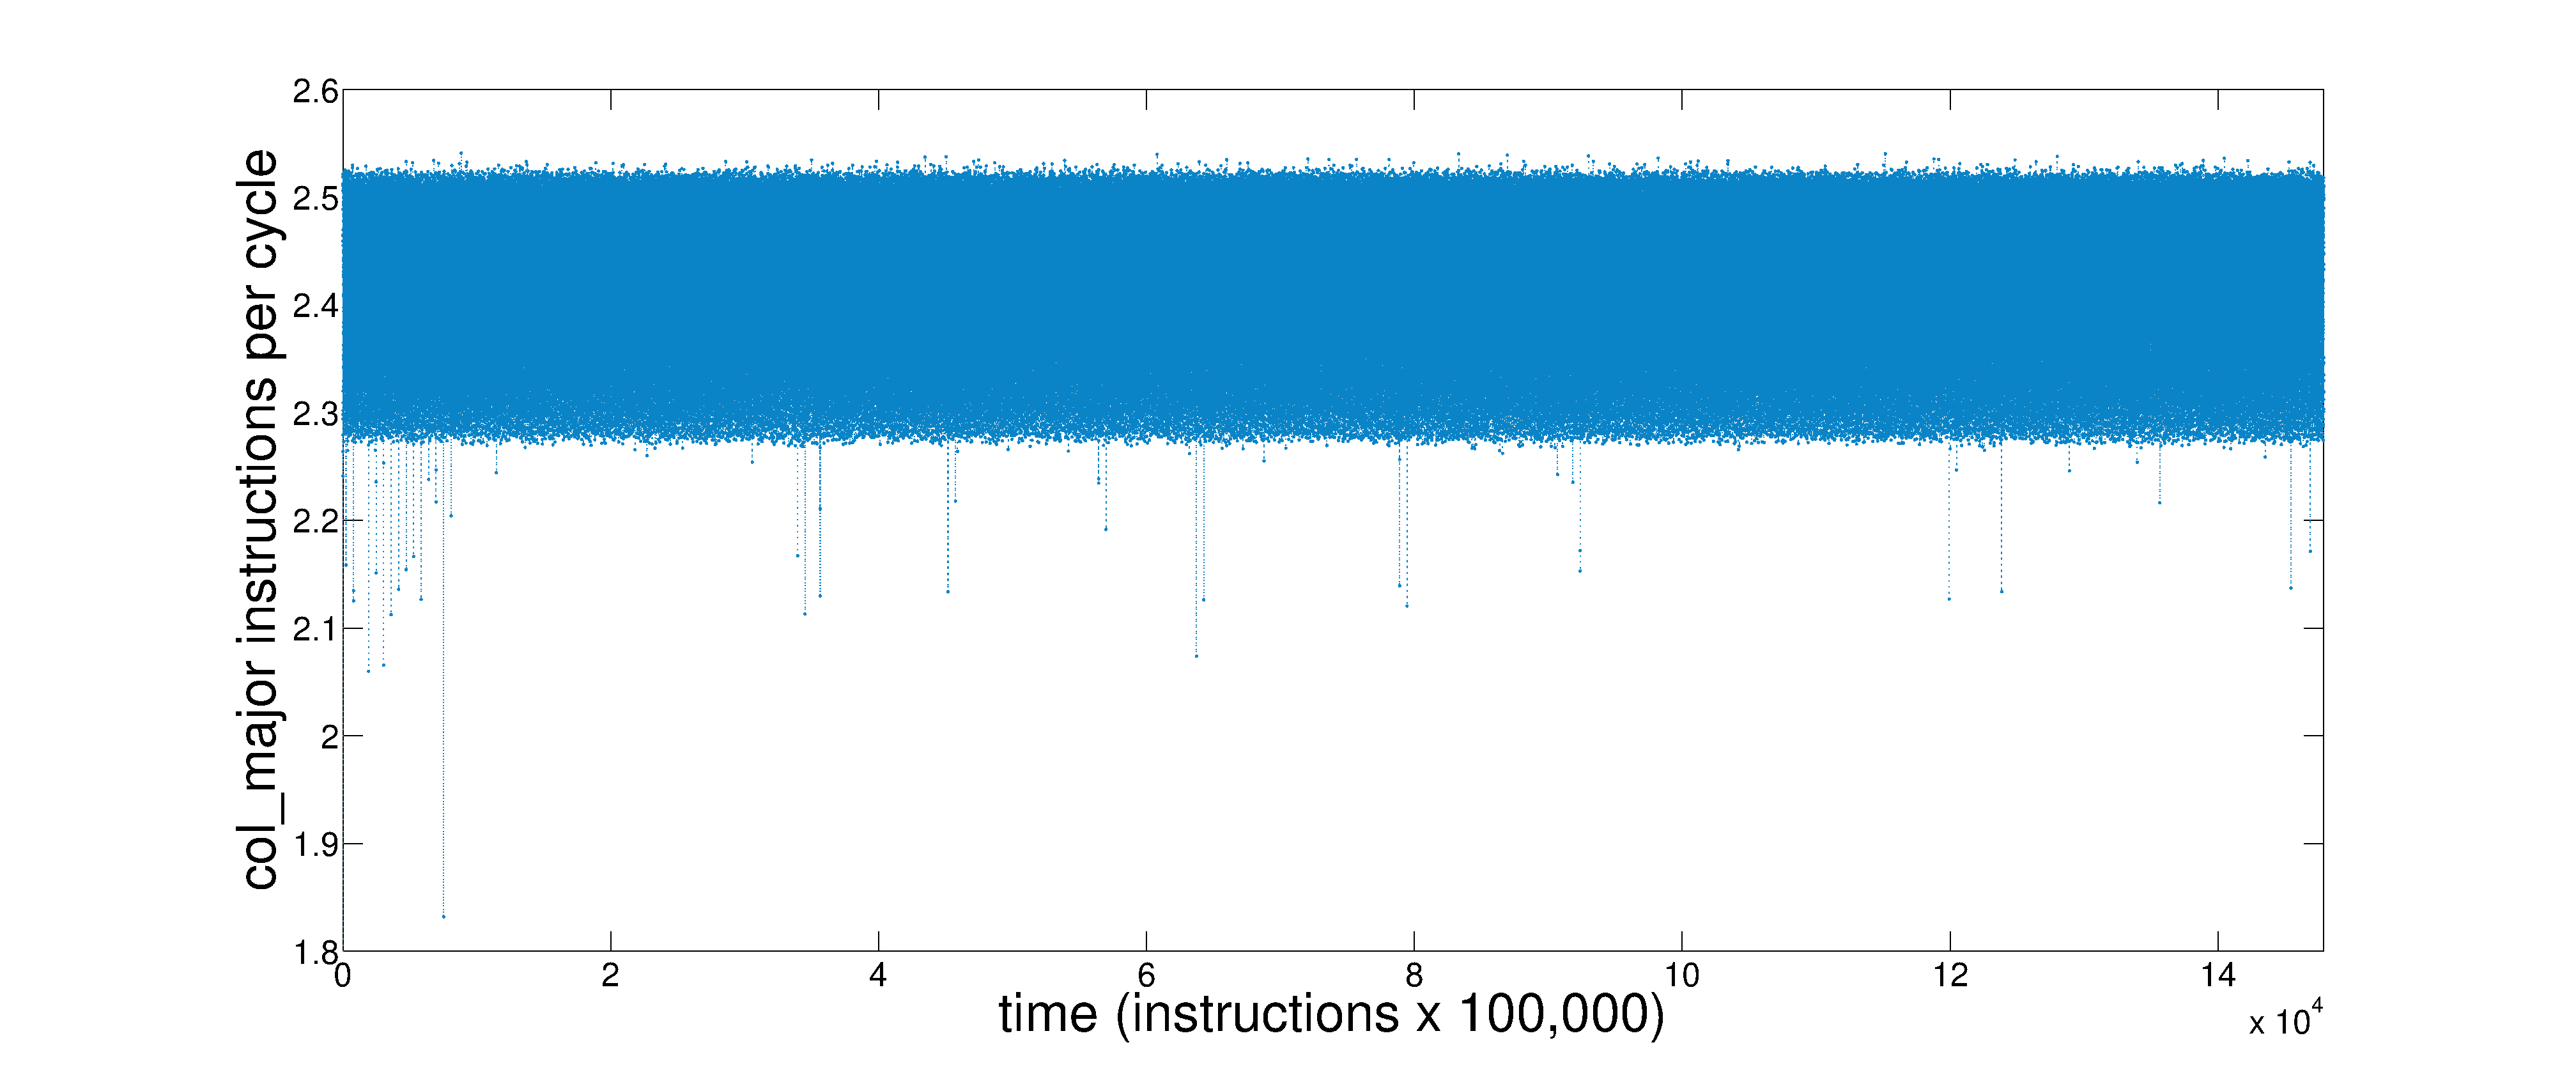
\includegraphics[width=\textwidth]{figs/colfullts}
                \caption{col IPC  Full Time Series}
                \label{fig:gull}
        \end{subfigure}%
        \newline
        ~ %add desired spacing between images, e. g. ~, \quad, \qquad etc.
          %(or a blank line to force the subfigure onto a new line)
        \begin{subfigure}[b]{\textwidth}
                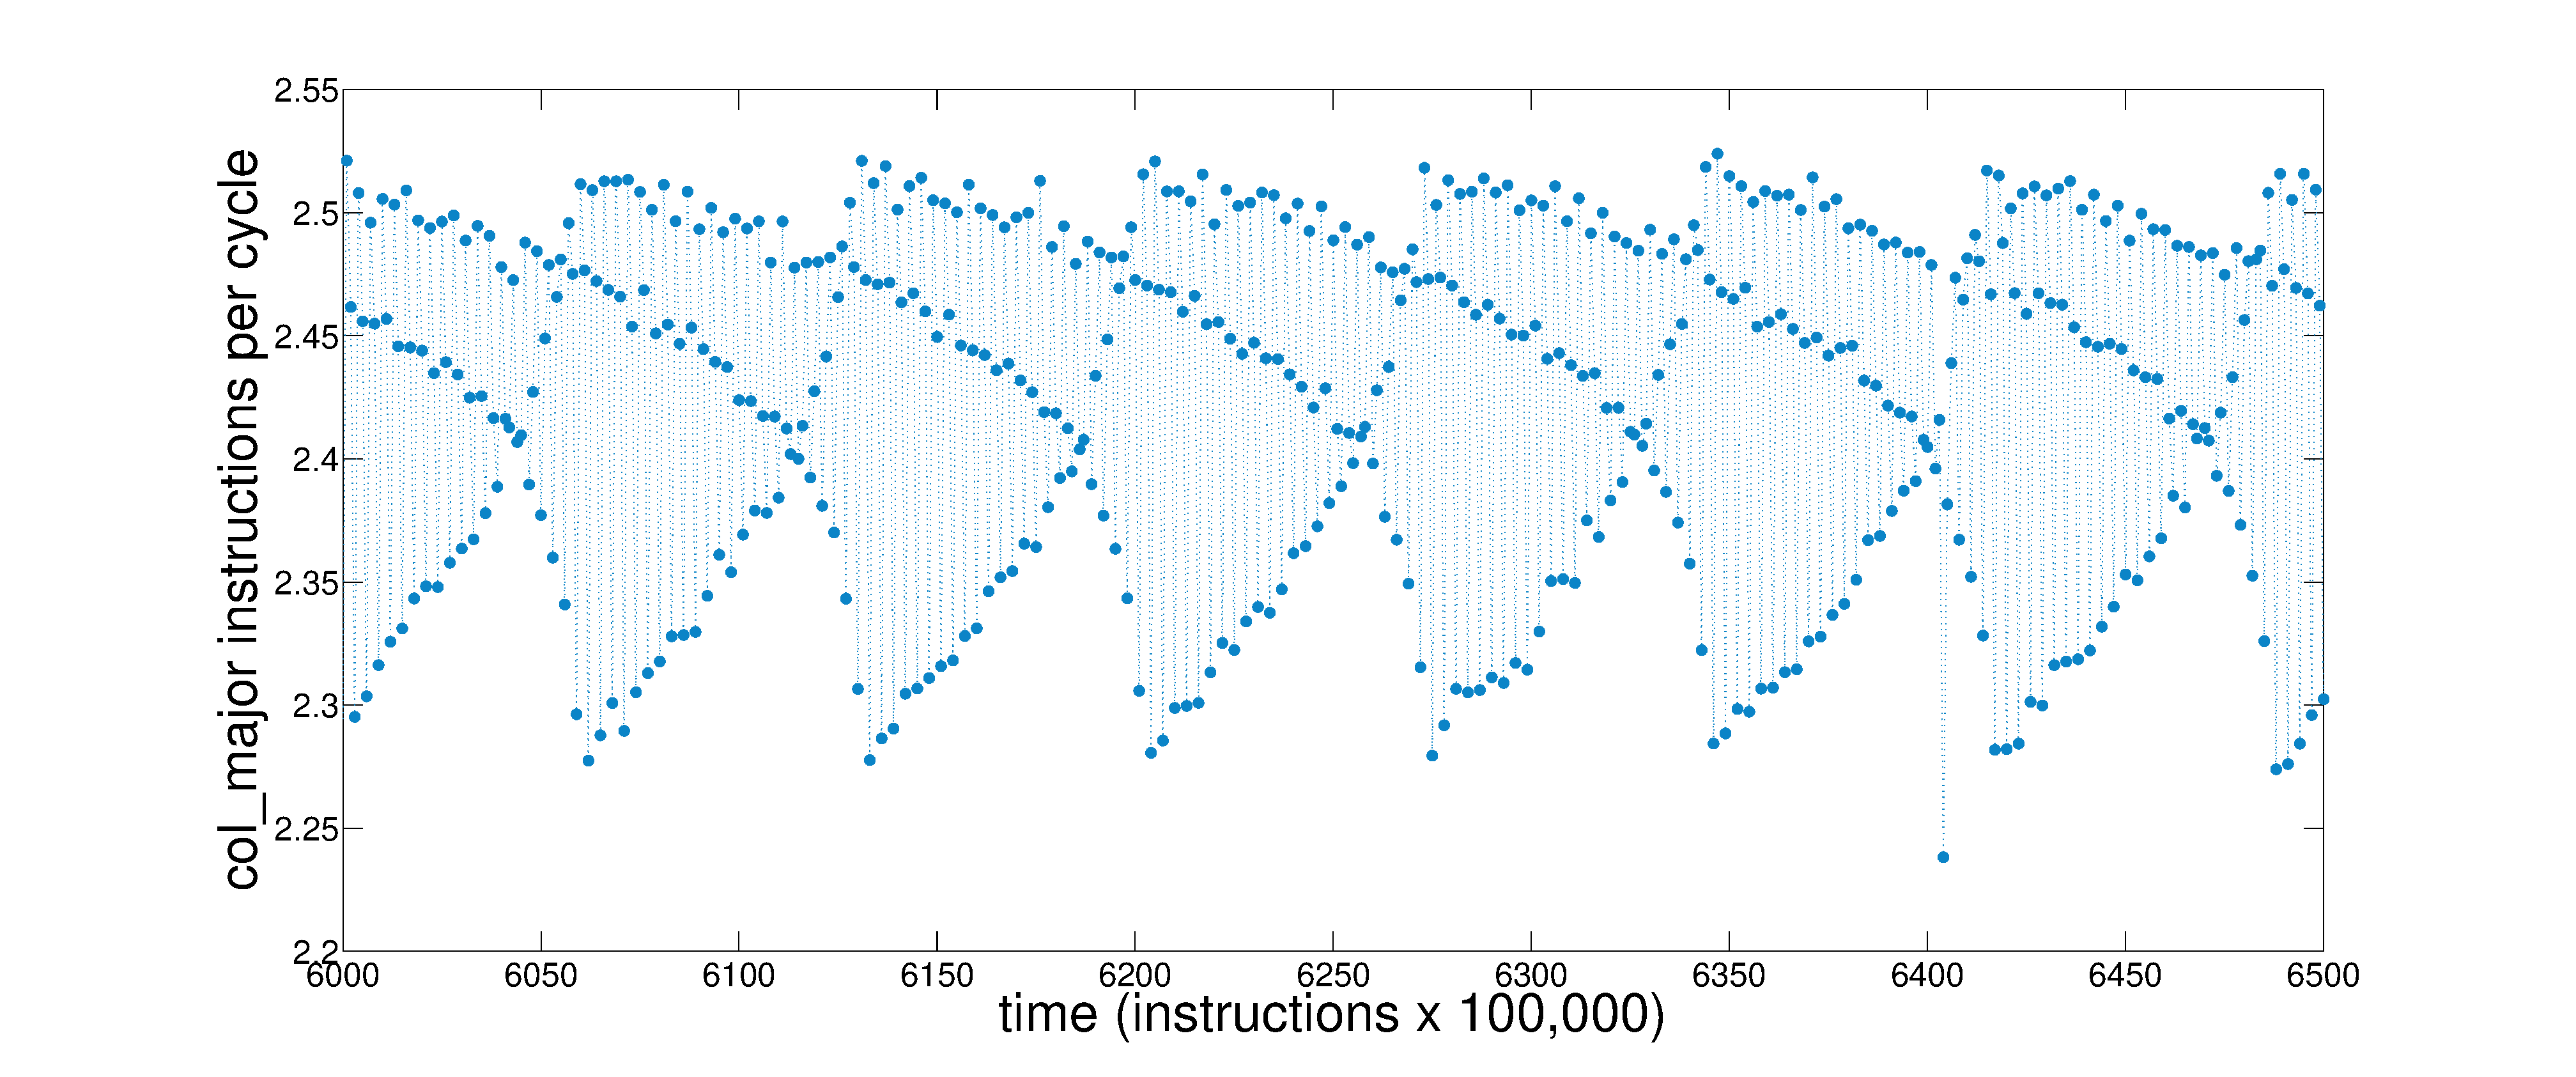
\includegraphics[width=\textwidth]{figs/colshortts}
                \caption{col IPC  Short Time Series for structure illustration}
                \label{fig:svdFullColored}
        \end{subfigure}

        ~ %add desired spacing between images, e. g. ~, \quad, \qquad etc.
          %(or a blank line to force the subfigure onto a new line)
         \caption{col  Time Series }\label{fig:svdFull}
\end{figure}

\begin{figure}
        \centering
        \begin{subfigure}{\textwidth}
                \includegraphics[width=\textwidth]{figs/colPredShortTS}
                \caption{col IPC  Full Time Series}
                \label{fig:gull}
        \end{subfigure}%
        \newline
        ~ %add desired spacing between images, e. g. ~, \quad, \qquad etc.
          %(or a blank line to force the subfigure onto a new line)
        \begin{subfigure}[b]{\textwidth}
                \includegraphics[width=\textwidth]{figs/colPredfullTS}
                \caption{col IPC  Short Time Series for structure illustration}
                \label{fig:svdFullColored}
        \end{subfigure}

        ~ %add desired spacing between images, e. g. ~, \quad, \qquad etc.
          %(or a blank line to force the subfigure onto a new line)
         \caption{col\_major Predictions }\label{fig:svdFull}
\end{figure}







\begin{figure}[htbp]
\begin{center}
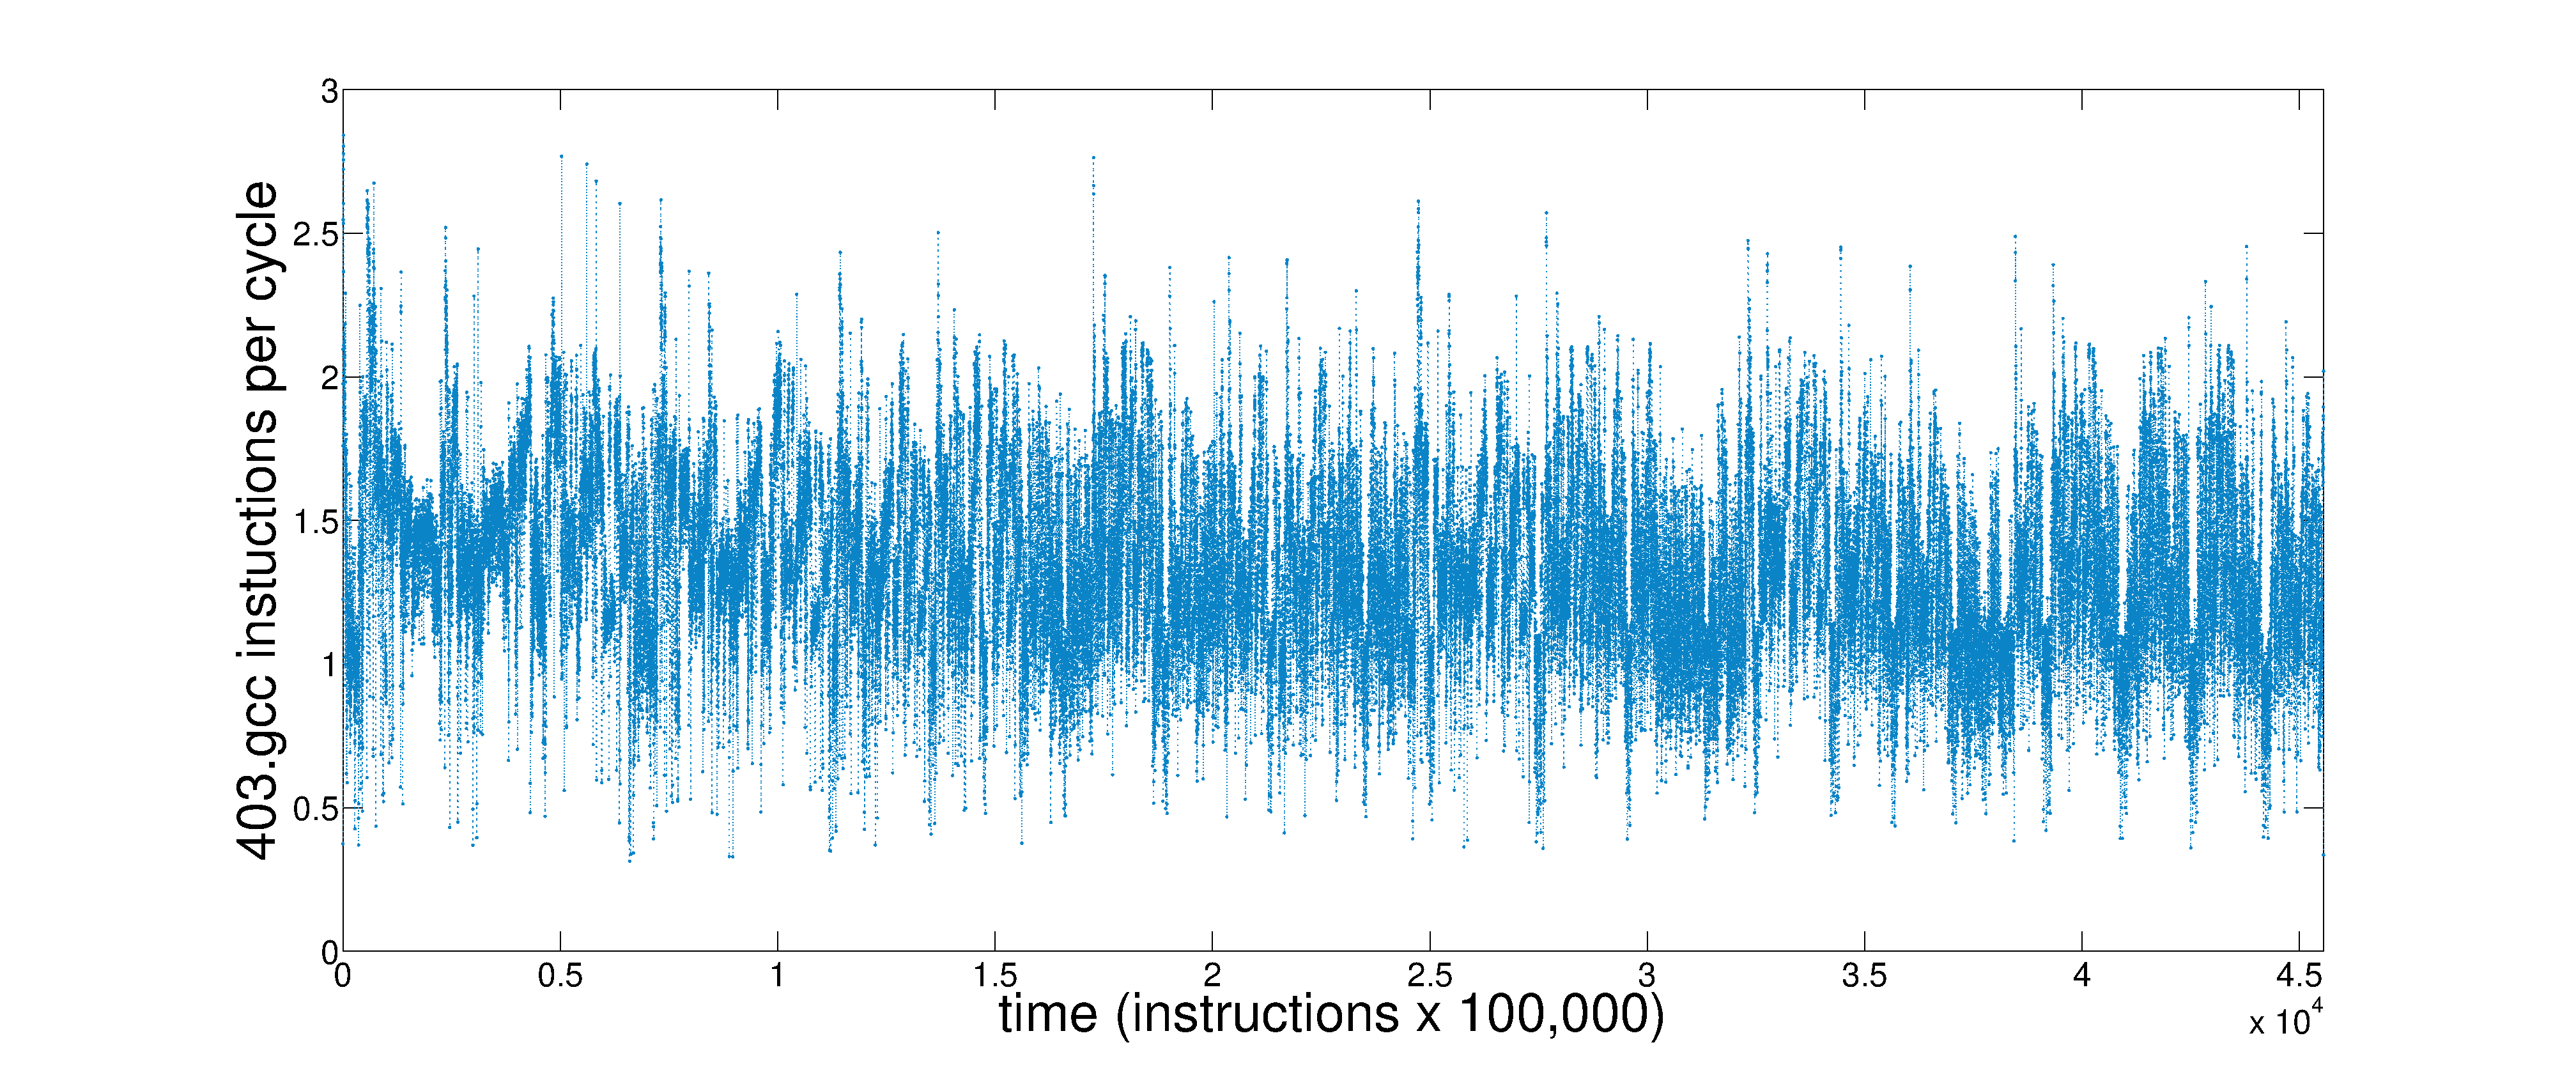
\includegraphics[width=\textwidth]{figs/gccfullts}\caption{403.gcc full time series}
\label{default}
\end{center}
\end{figure}





\begin{figure}[htbp]
\begin{center}
\includegraphics[width=\textwidth]{figs/svd_mutuals}\caption{SVD mutuals for full and regimes}
\label{default}
\end{center}
\end{figure}






\begin{figure}[htbp]
\begin{center}
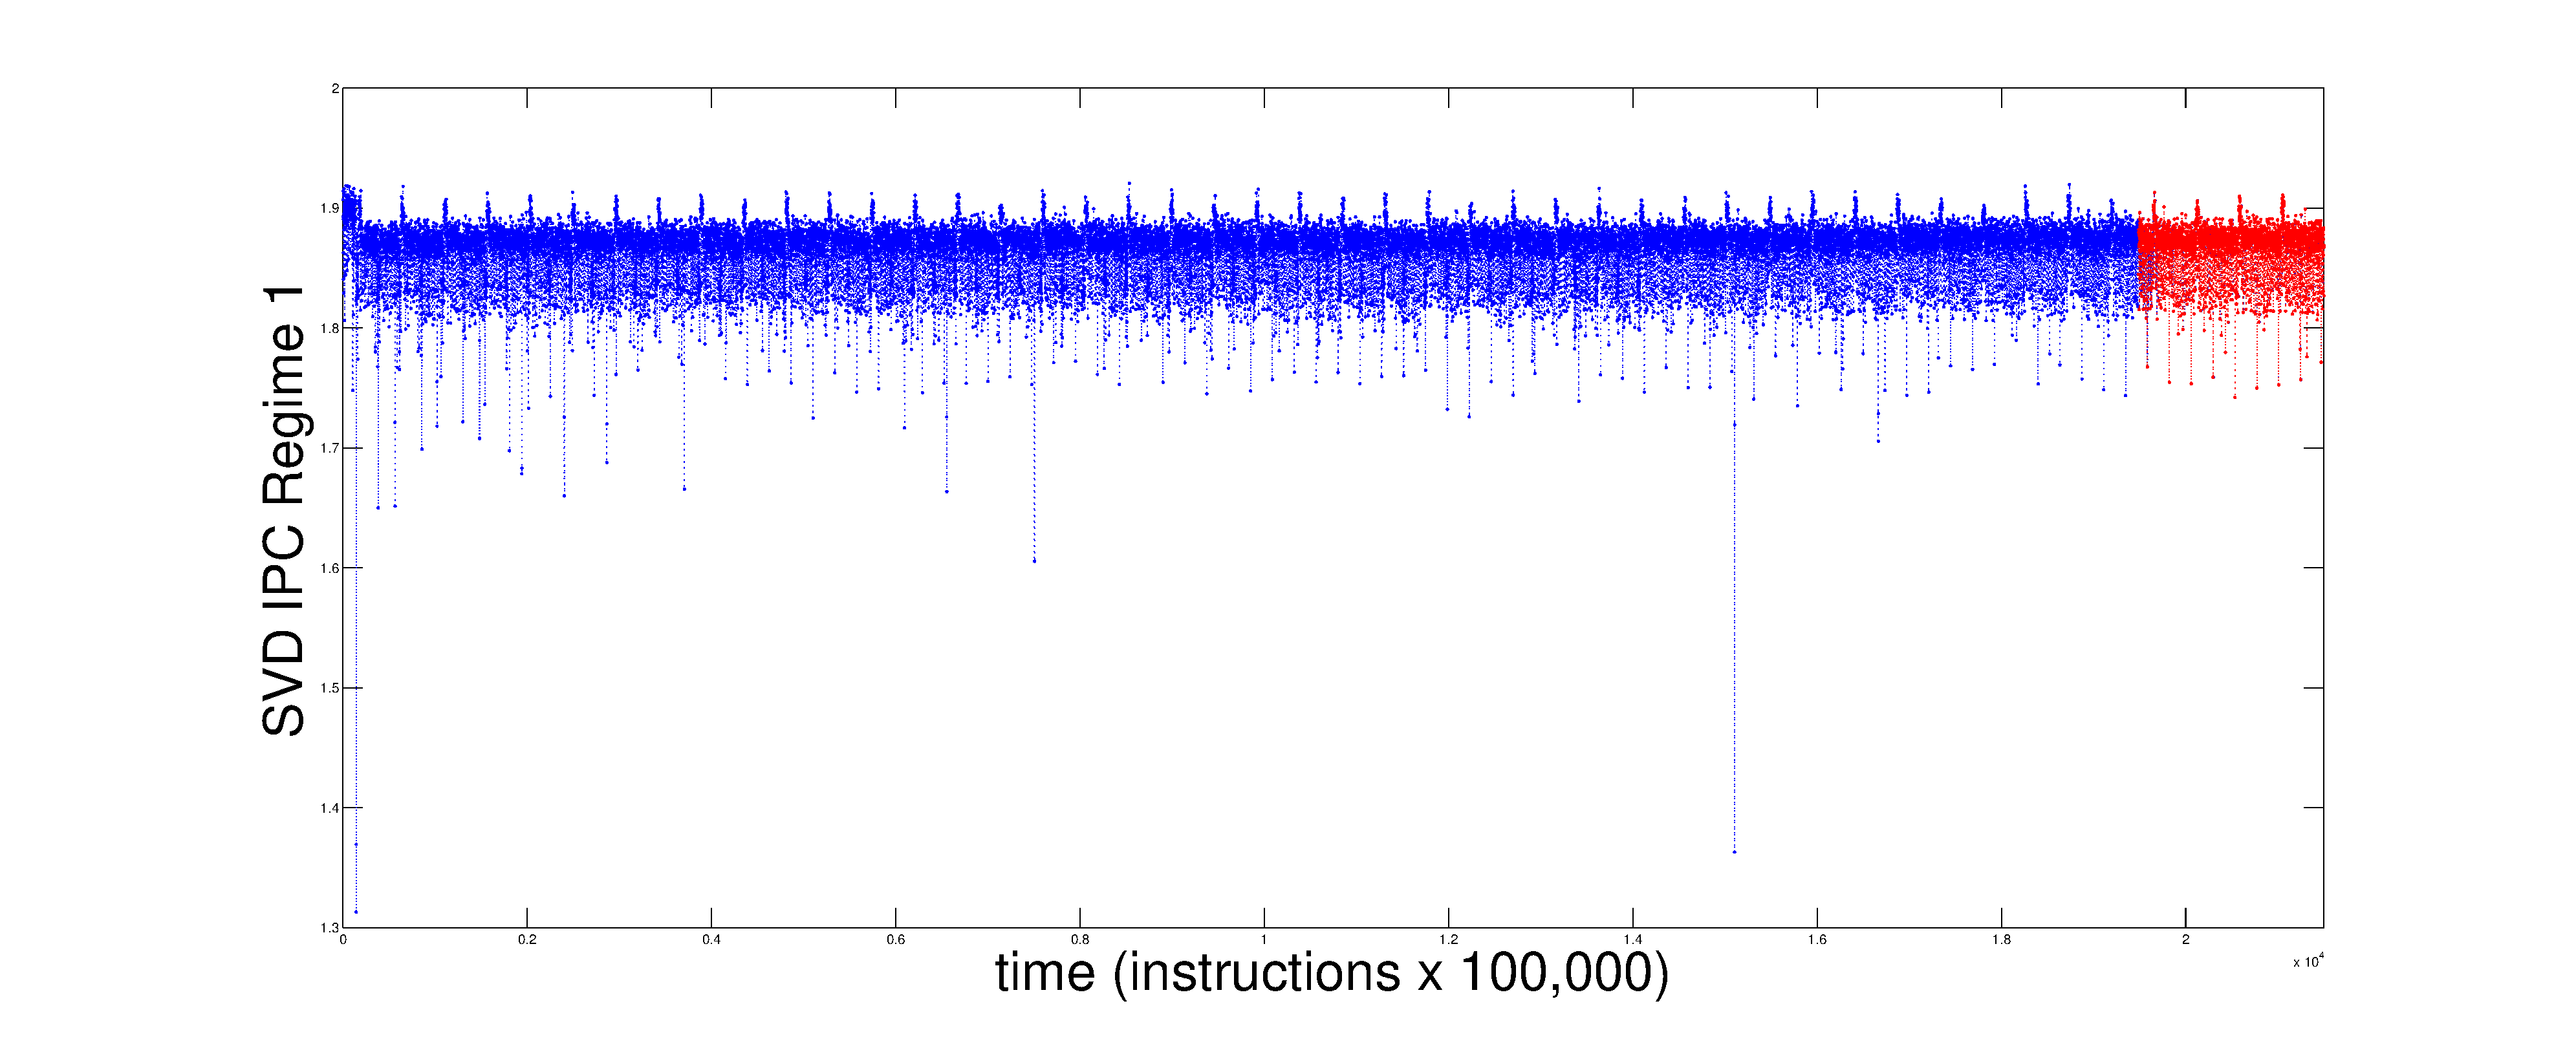
\includegraphics[width=\textwidth]{figs/regime1}\caption{SVD IPC Regime 1 Time Series}
\label{default}
\end{center}
\end{figure}


\begin{figure}[htbp]
\begin{center}
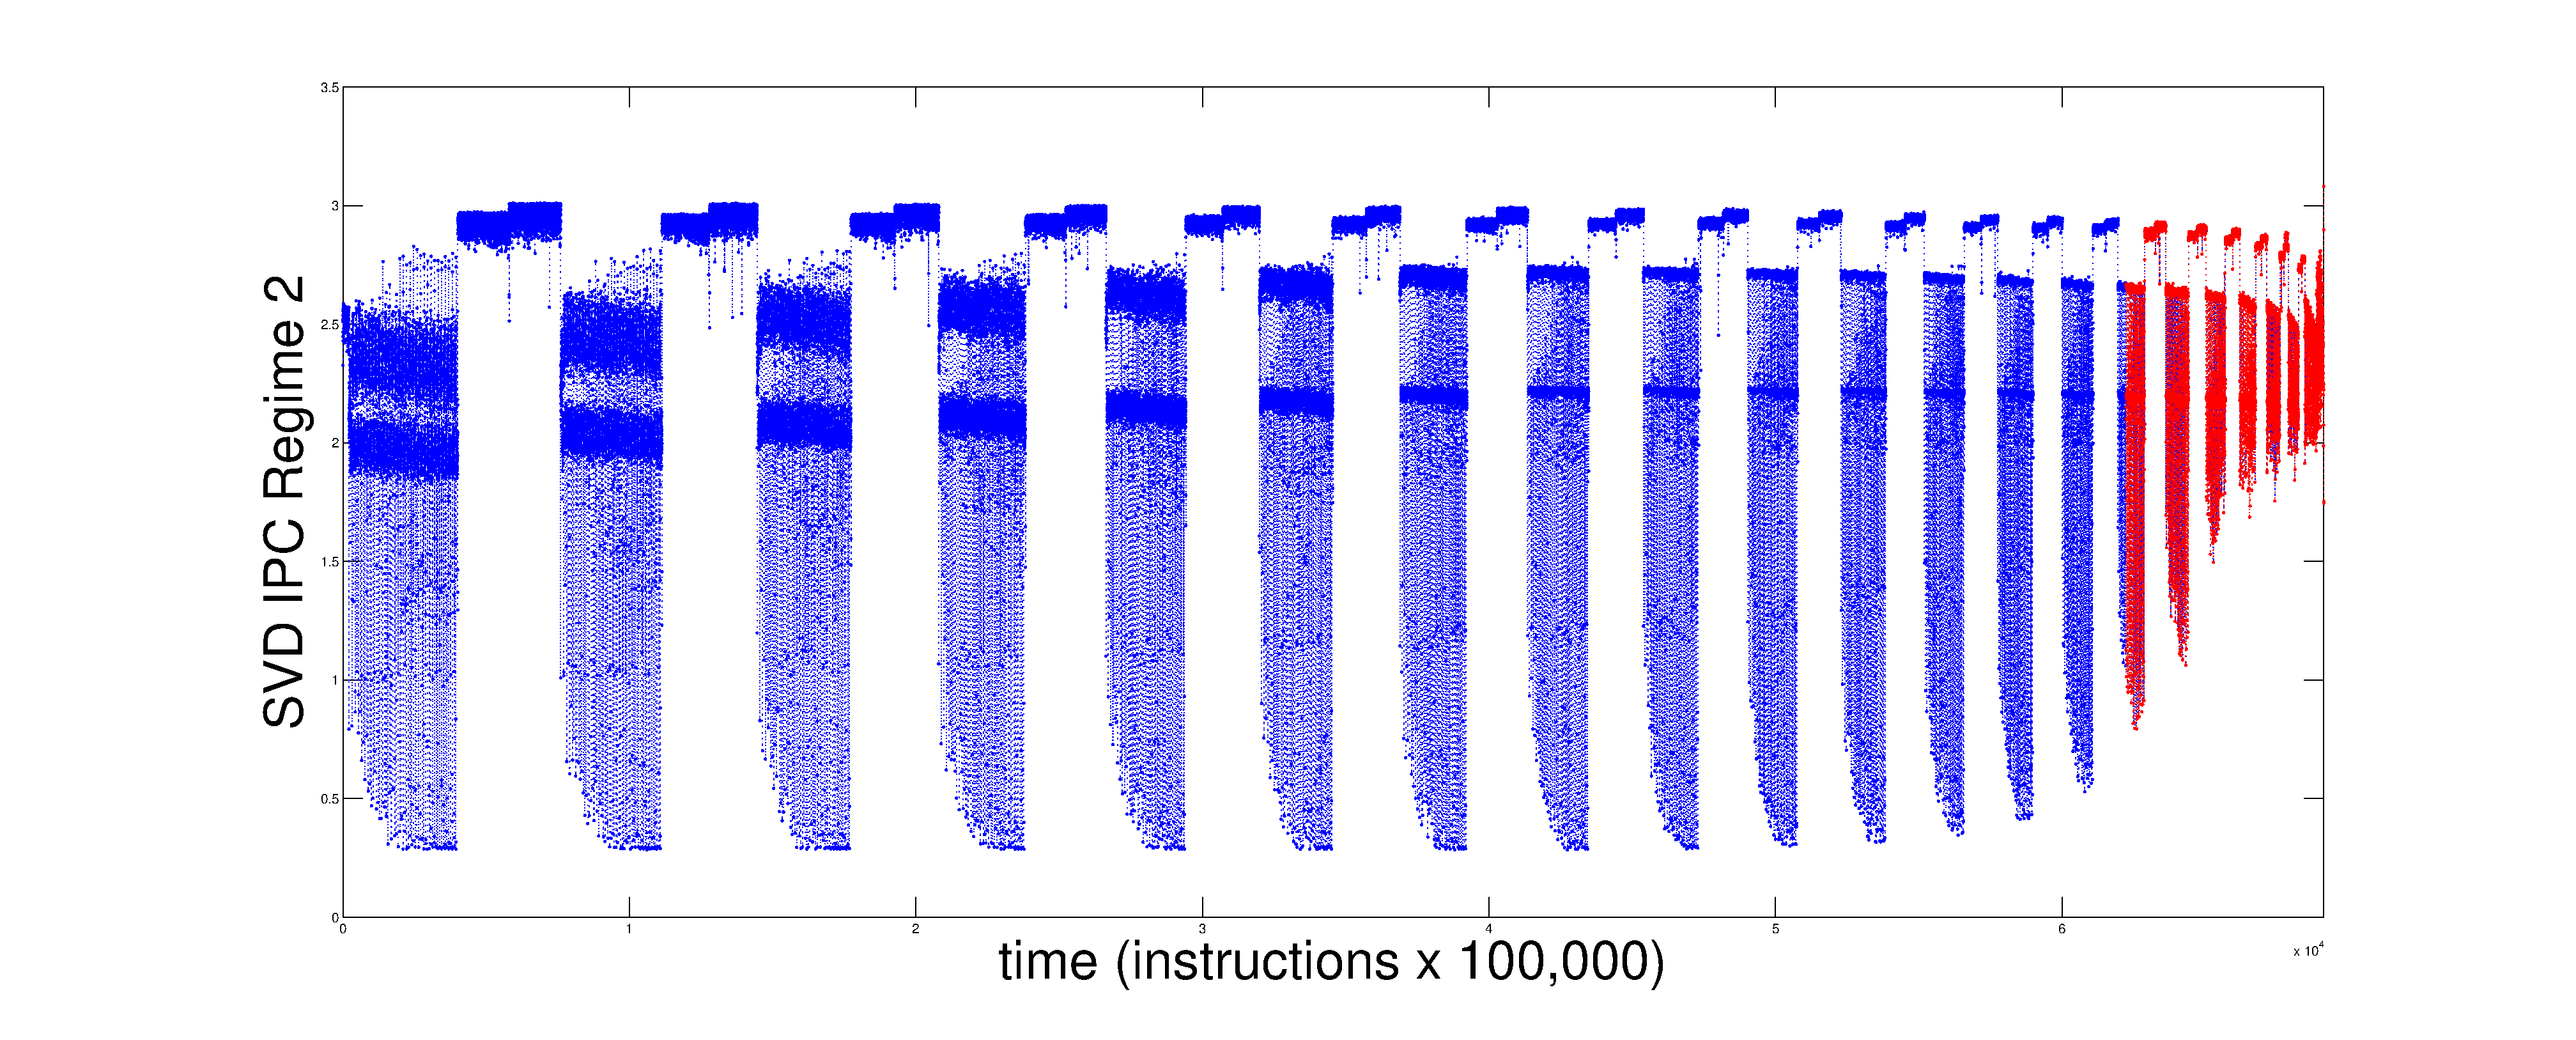
\includegraphics[width=\textwidth]{figs/regime2}\caption{SVD IPC Regime 2 Time Series}
\label{default}
\end{center}
\end{figure}


%\begin{figure}[htbp]
%\begin{center}
%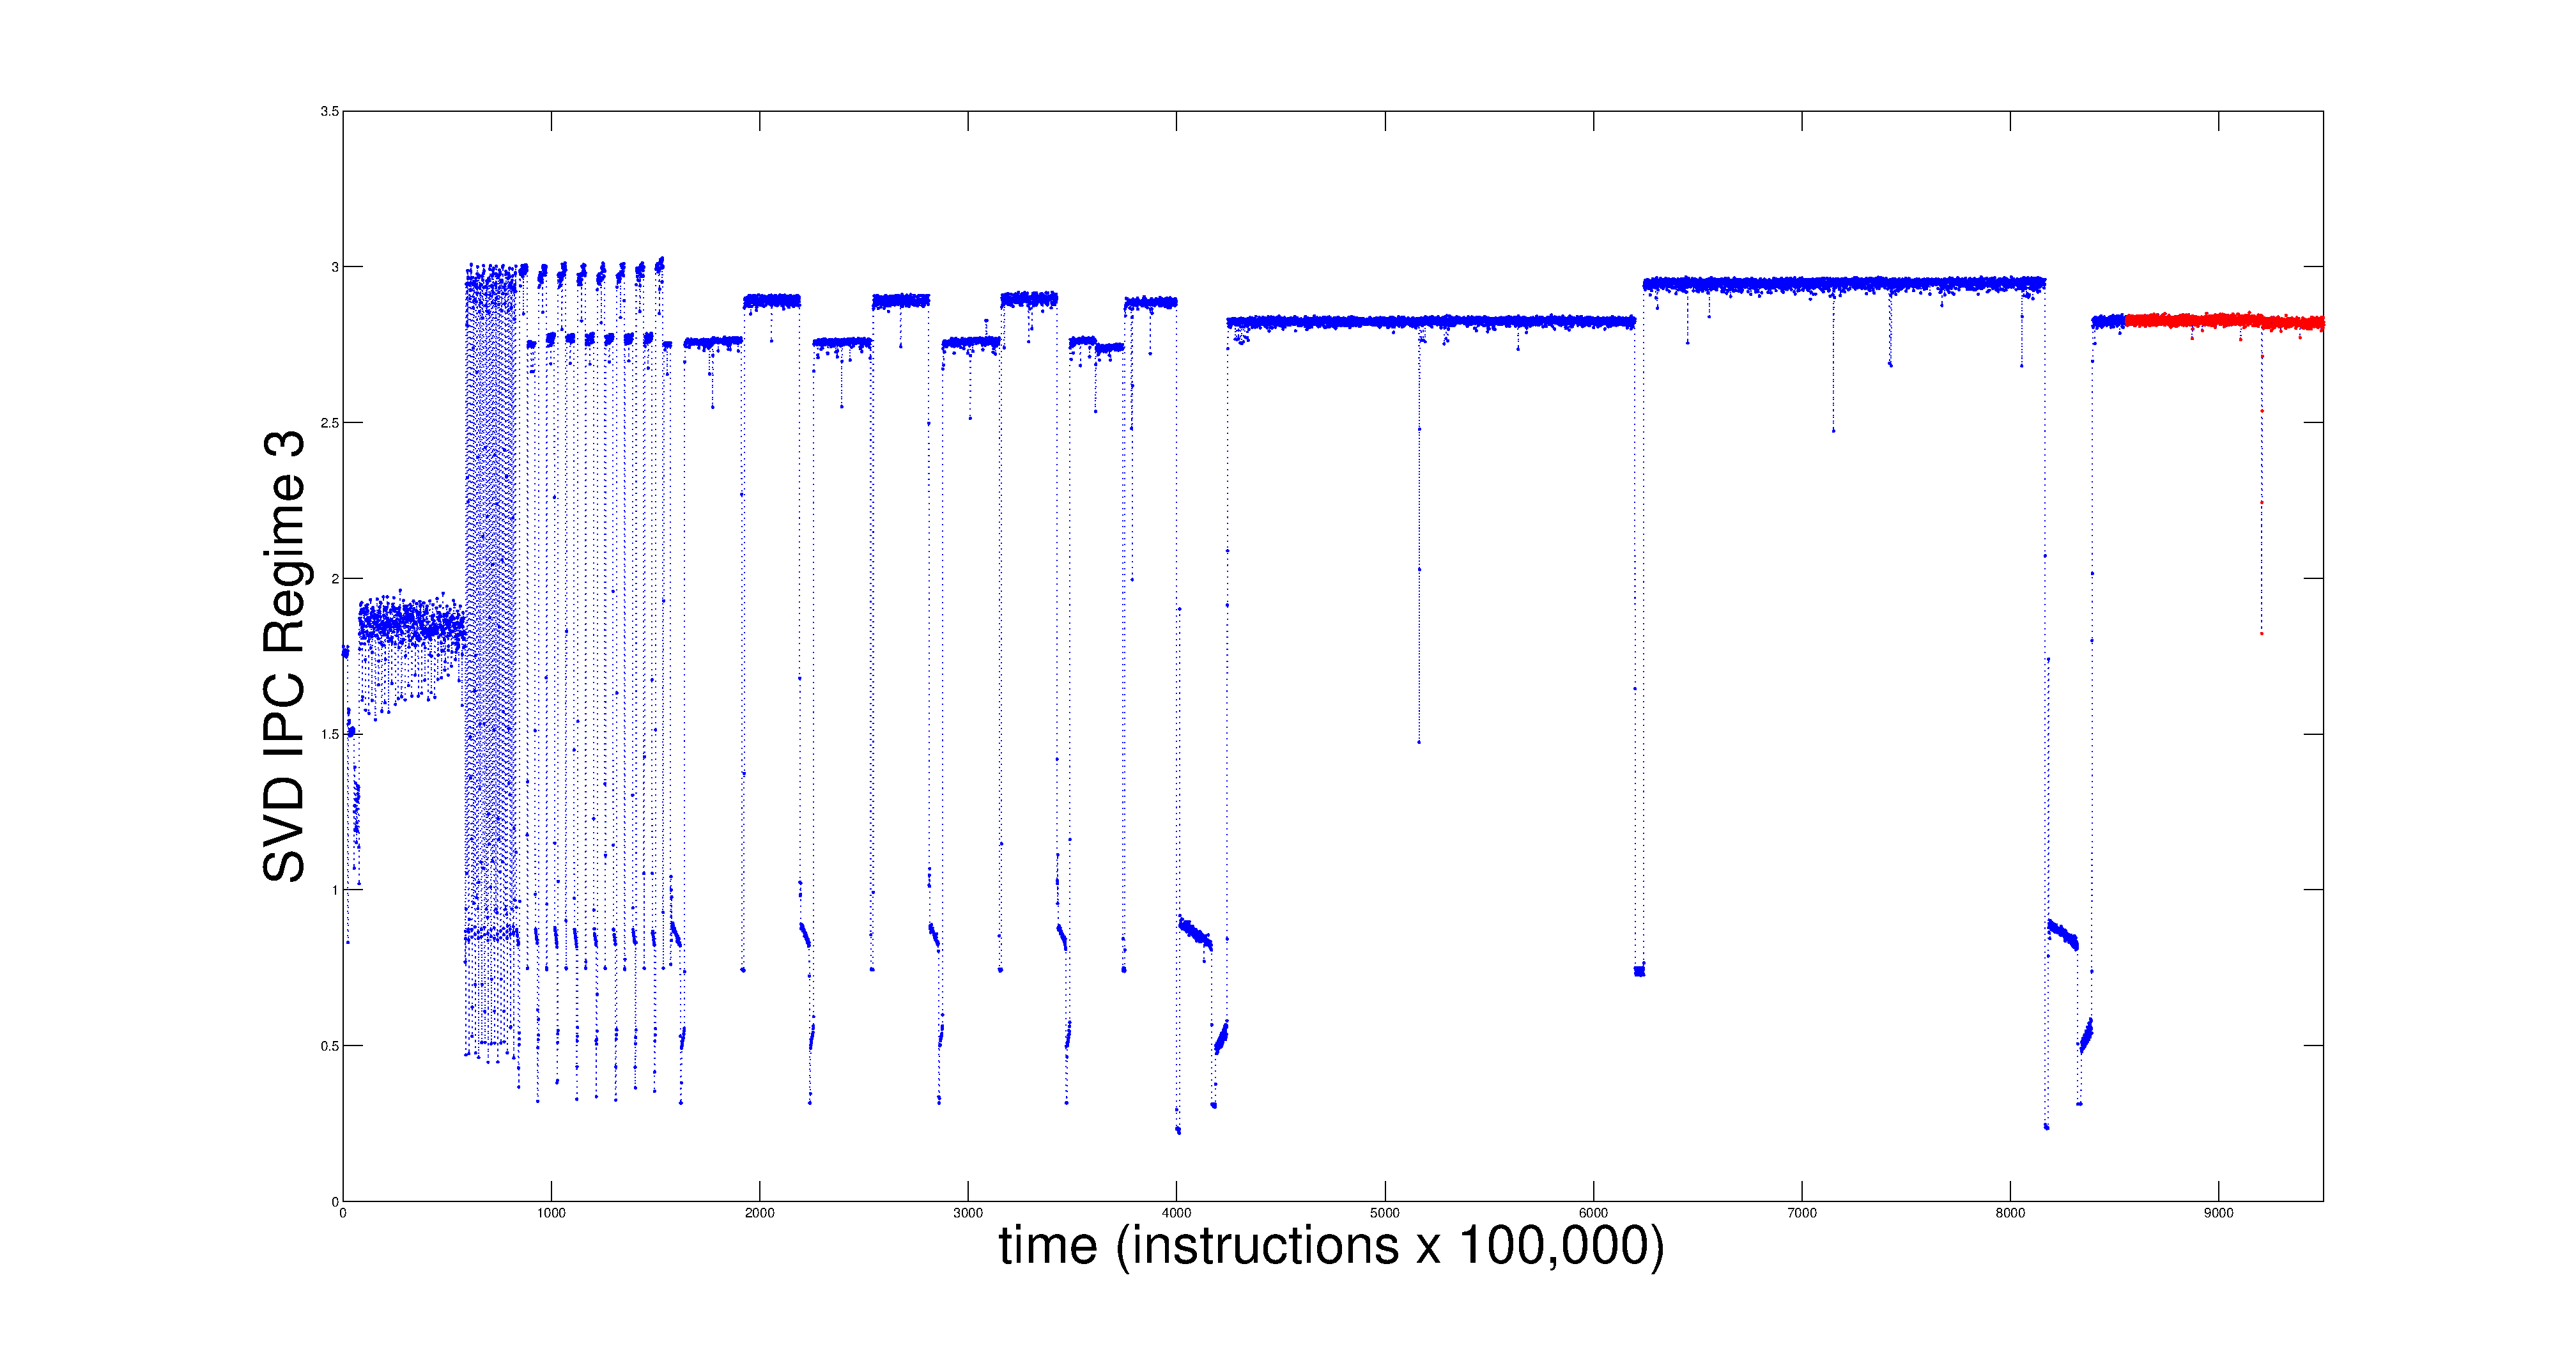
\includegraphics[width=\textwidth]{figs/regime3}\caption{SVD IPC Regime 3 Time Series}
%\label{default}
%\end{center}
%\end{figure}

%\begin{figure}[htbp]
%\begin{center}
%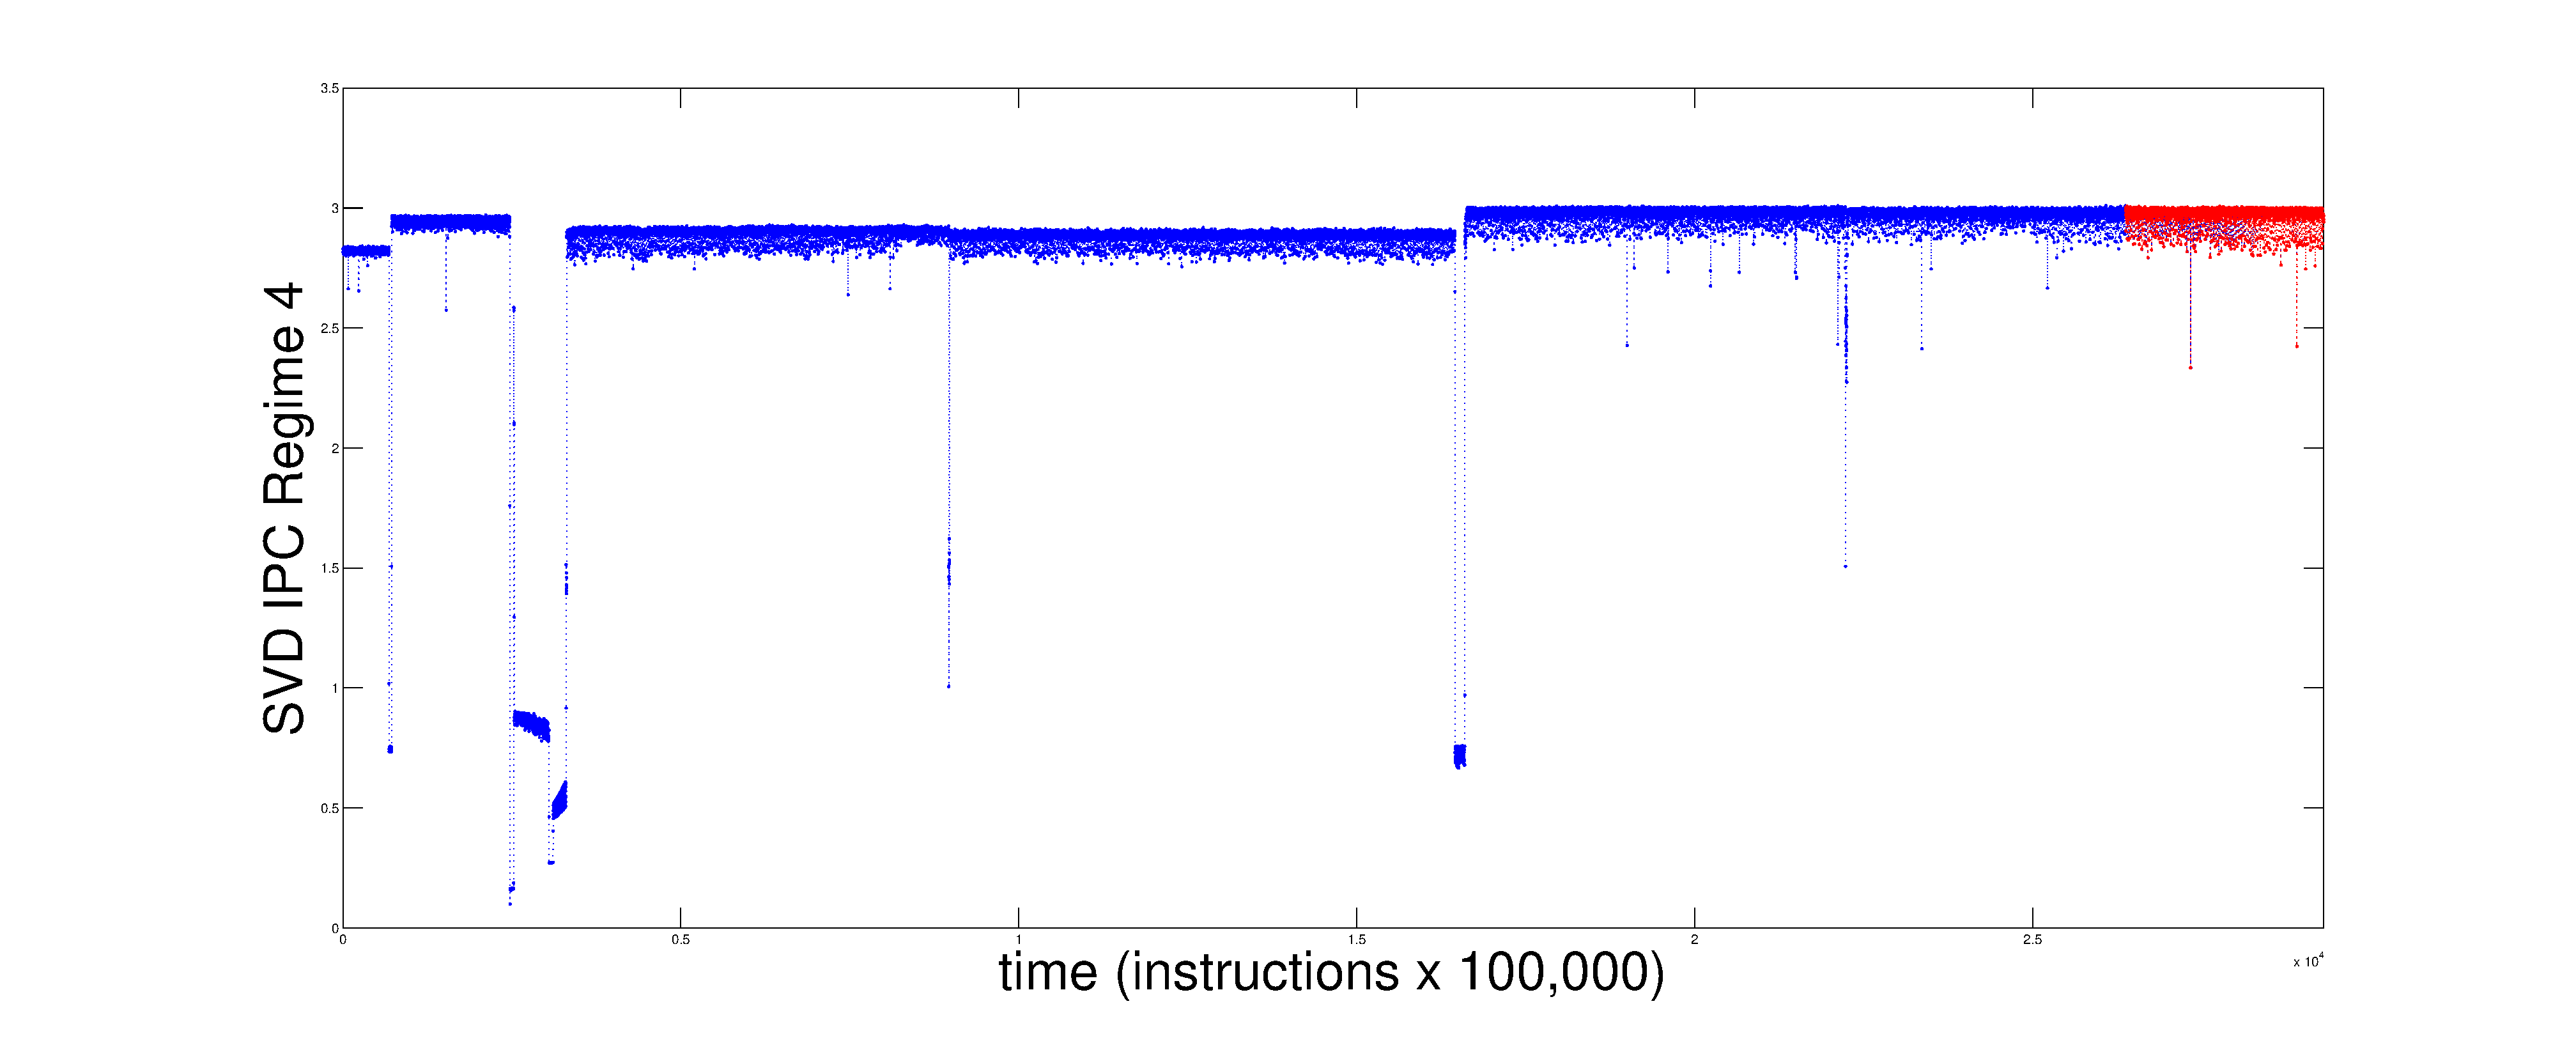
\includegraphics[width=\textwidth]{figs/regime4}\caption{SVD IPC Regime 4 Time Series}
%\label{default}
%\end{center}
%\end{figure}

\begin{figure}[htbp]
\begin{center}
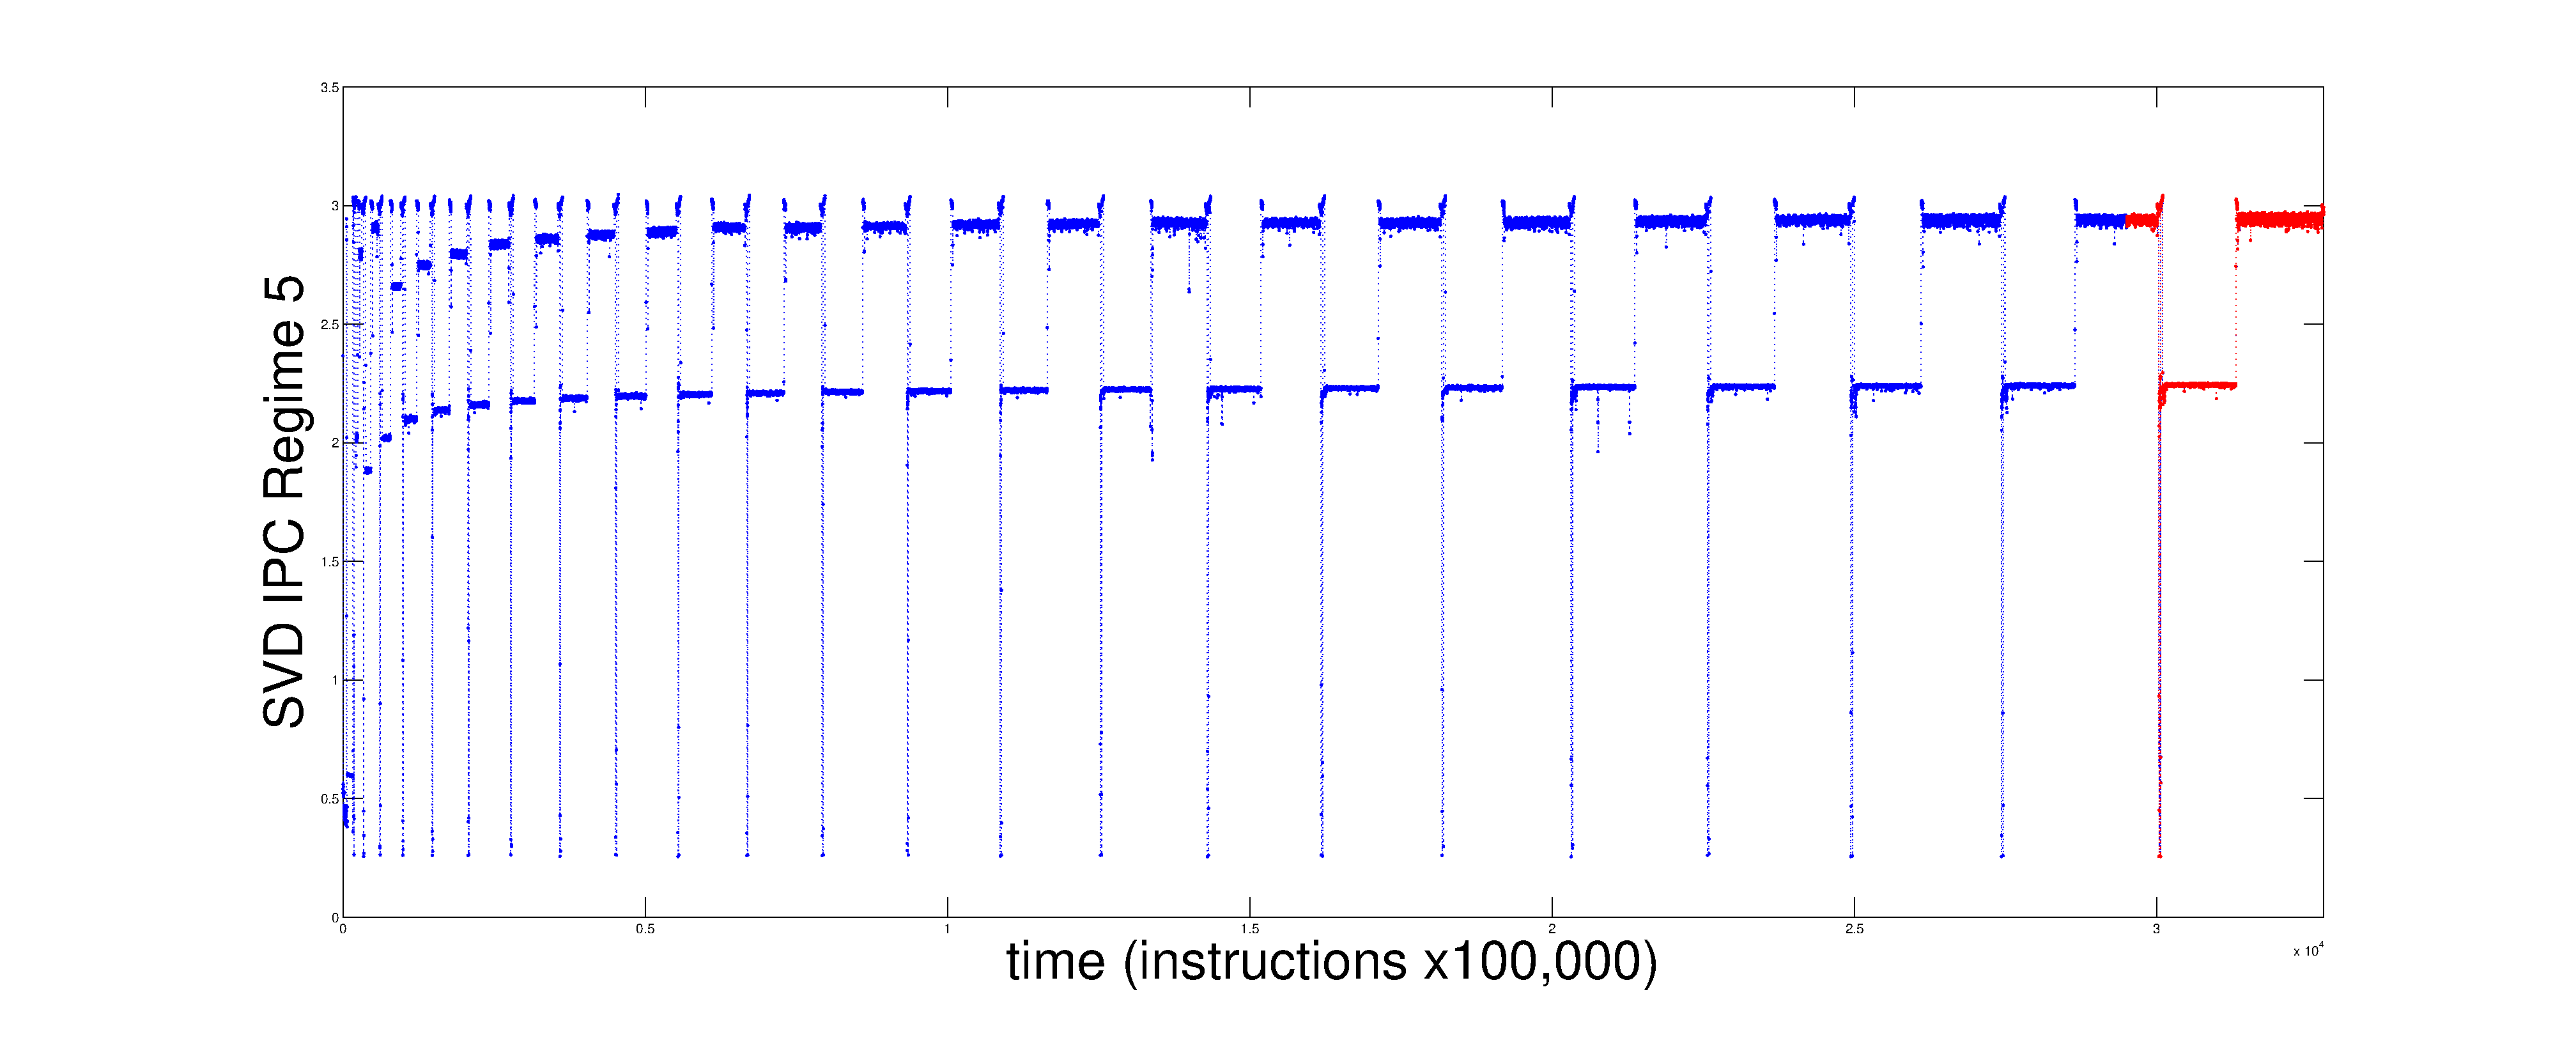
\includegraphics[width=\textwidth]{figs/regime5}\caption{SVD IPC Regime 5 Time Series}
\label{default}
\end{center}
\end{figure}

\begin{figure}[htbp]
\begin{center}
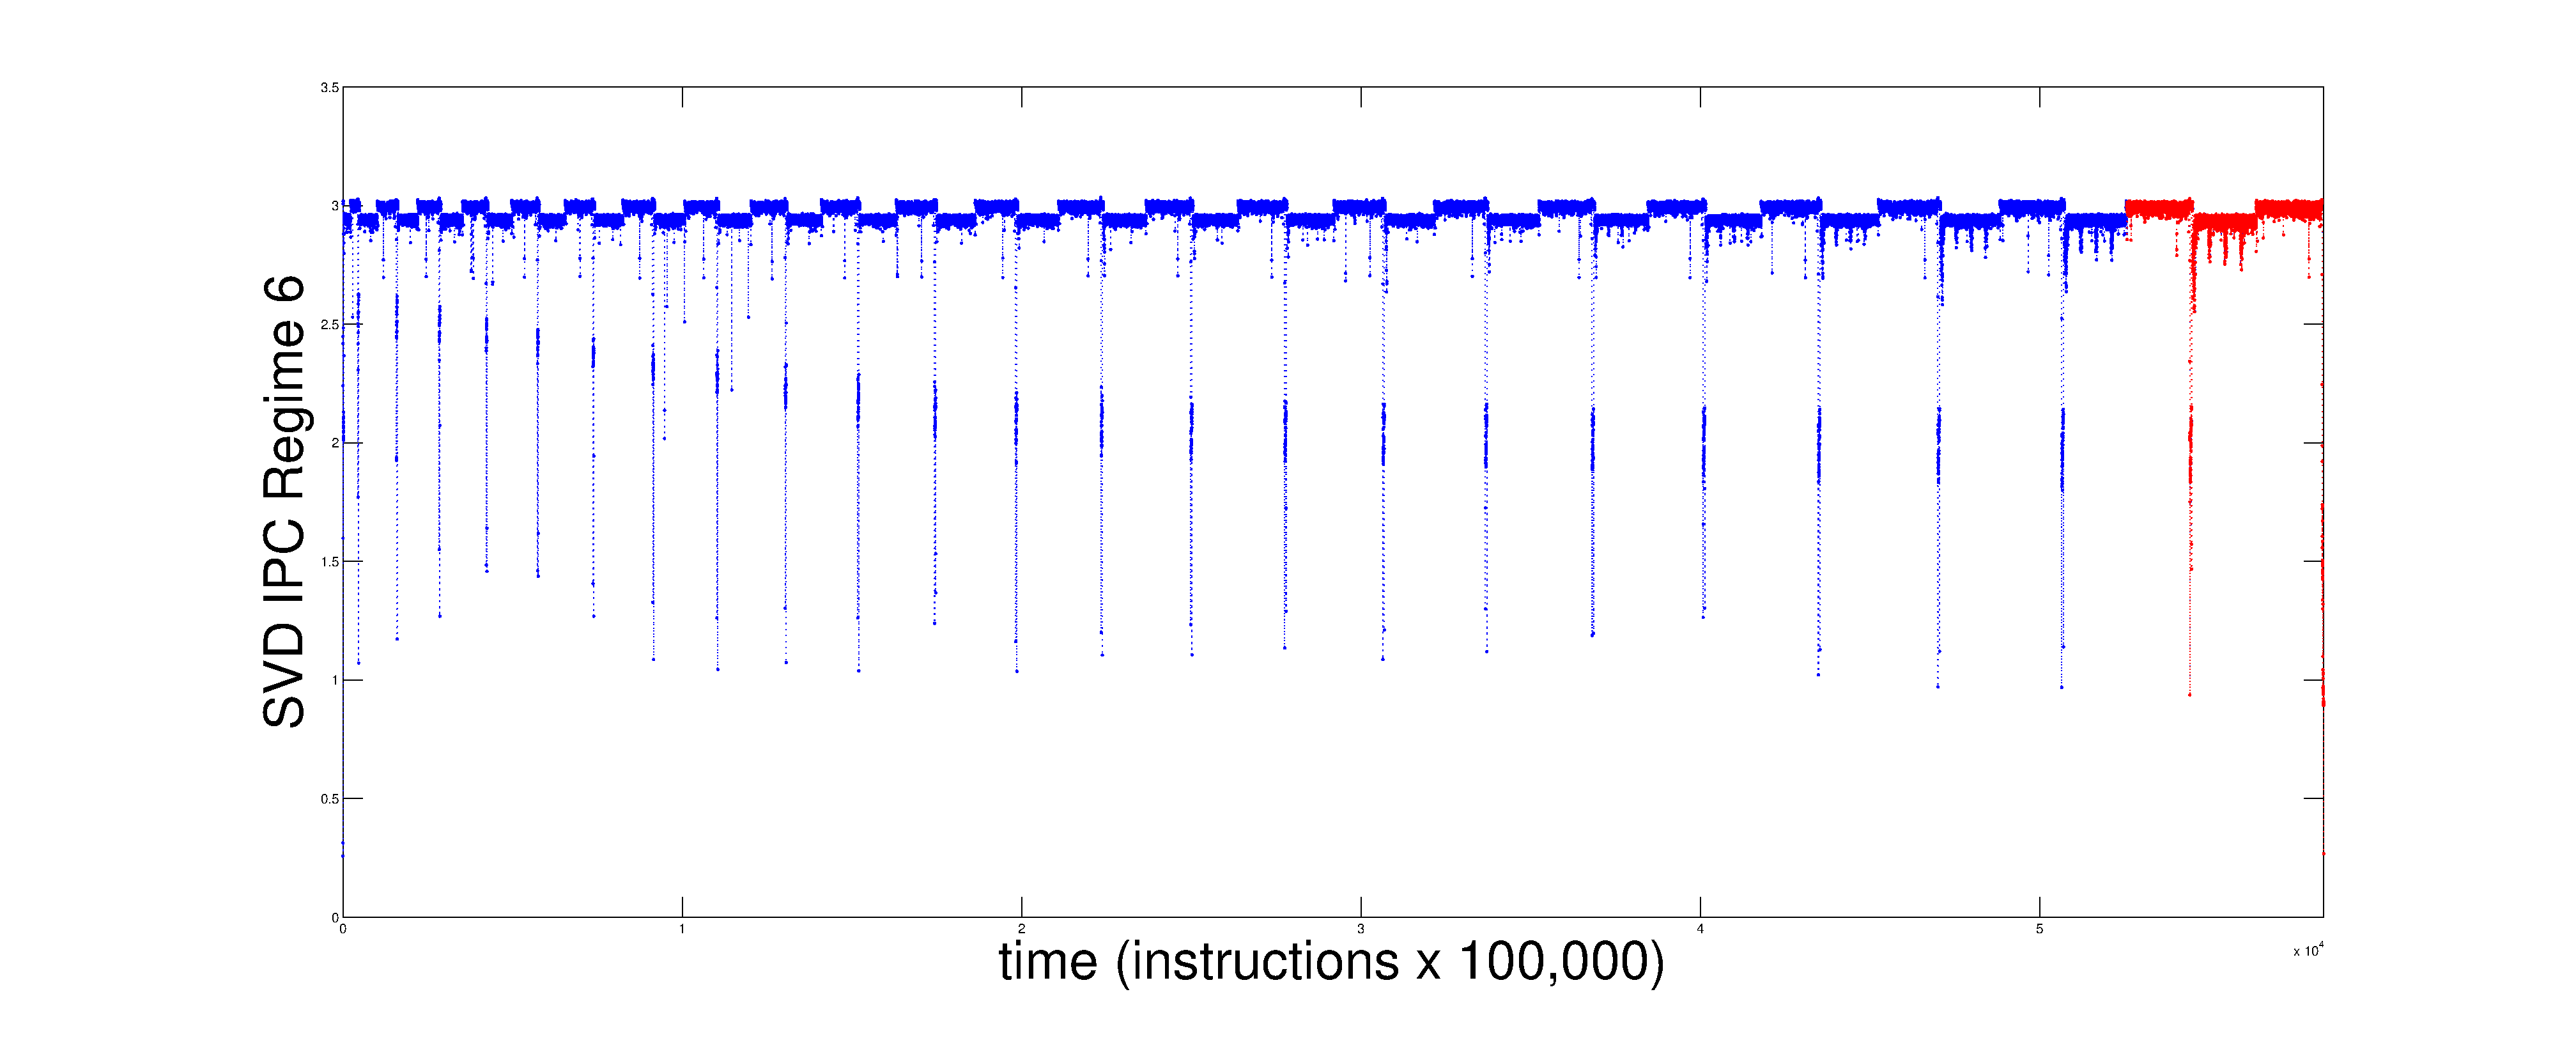
\includegraphics[width=\textwidth]{figs/regime6}\caption{SVD IPC Regime 6 Time Series}
\label{default}
\end{center}
\end{figure}


\begin{figure}[htbp]
  \centering
  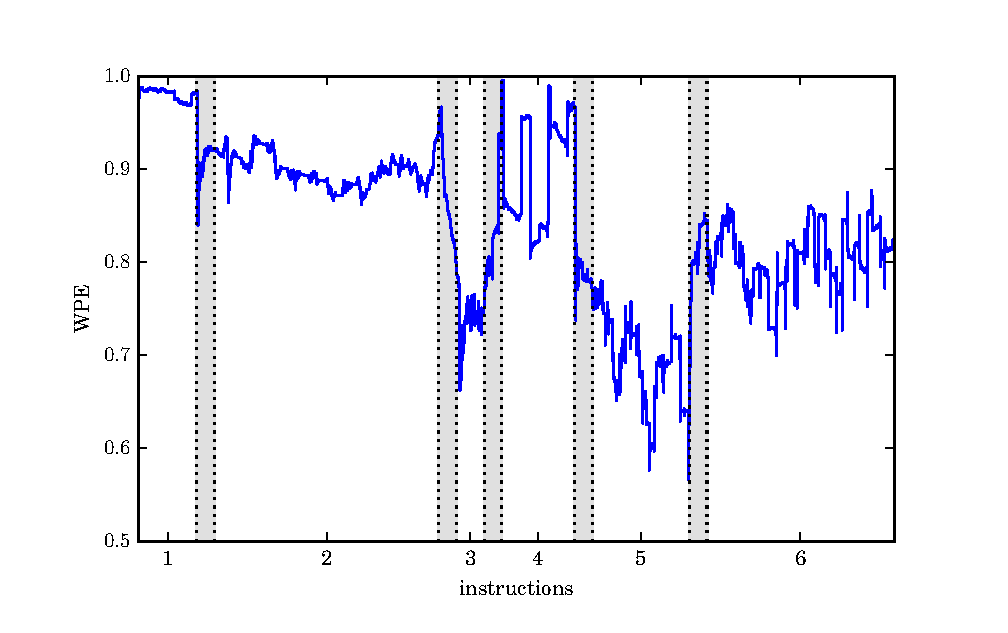
\includegraphics[width=0.95\textwidth]{figs/SVD_wwpe}
  \caption{The weighted permutation entropy of one run of SVD. The gray bands
    are regions where the window overlaps regimes. The window size used is
    $5,000 \times 100,000$ instructions and the word length is $4$.}
  \label{fig:wwpe}
\end{figure}

\begin{figure}[htbp]
  \centering
  \includegraphics[width=0.95\textwidth]{figs/prediction_vs_entropy}
  \caption{The improvement of LMA over na\"{i}ve vs weighted permutation entropy.
  For each of these, the word length used is $5$.}
  \label{fig:pred_vs_ent}
\end{figure}






\section*{Acknowledgment}
This work was partially supported by NSF grant \#CMMI-1245947 and ARO
grant \#W911NF-12-1-0288.

\bibliographystyle{unsrt}
\bibliography{bibliofile}


\end{document}
